% ******************************************************** %
%              TEMPLATE DE INFORME ORGA2 v0.1              %
% ******************************************************** %
% ******************************************************** %
%                                                          %
% ALGUNOS PAQUETES REQUERIDOS (EN UBUNTU):                 %
% ========================================
%                                                          %
% texlive-latex-base                                       %
% texlive-latex-recommended                                %
% texlive-fonts-recommended                                %
% texlive-latex-extra?                                     %
% texlive-lang-spanish (en ubuntu 13.10)                   %
% ******************************************************** %


\documentclass[a4paper]{article}
\usepackage[spanish]{babel}
\usepackage[utf8]{inputenc}
\usepackage{charter}   % tipografia
\usepackage{graphicx}
\usepackage[table,xcdraw,dvipsnames]{xcolor}
%\usepackage{makeidx}
\usepackage{paralist} %itemize inline

\usepackage{float}
\usepackage{amsmath, amsthm, amssymb}
\usepackage{amsfonts}
%\usepackage{sectsty}
%\usepackage{charter}
%\usepackage{wrapfig}
\usepackage{listingsutf8}

% \setcounter{secnumdepth}{2}
\usepackage{underscore}
\usepackage{caratula}
\usepackage{url}
%\usepackage[superscript,biblabel]{cite}
%\usepackage{dibujitos}

\usepackage{ textcomp }

\usepackage{amssymb}
\usepackage{hyperref}


\graphicspath{ {img/} {../graph/} }

% ********************************************************* %
% ~~~~~~~~              Code snippets             ~~~~~~~~~ %
% ********************************************************* %

\usepackage{color} % para snipets de codigo coloreados
\usepackage{fancybox}  % para el sbox de los snipets de codigo

\definecolor{litegrey}{gray}{0.94}

\newenvironment{codesnippet}{%
	\begin{Sbox}\begin{minipage}{\textwidth}\sffamily\small}%
	{\end{minipage}\end{Sbox}%
		\begin{center}%
		\vspace{-0.4cm}\colorbox{litegrey}{\TheSbox}\end{center}\vspace{0.3cm}}

\definecolor{mygreen}{rgb}{0,0.6,0}
\definecolor{mygray}{rgb}{0.5,0.5,0.5}
\definecolor{mymauve}{rgb}{0.58,0,0.82}

\lstset{ %
  backgroundcolor=\color{litegrey},
  basicstyle=\footnotesize,
  breakatwhitespace=true,
  breaklines=true,
  captionpos=b,                    % sets the caption-position to bottom
  mathescape=true,
  keepspaces=true,
  language=Python,
  showspaces=false,
  tabsize=2,                       % sets default tabsize to 2 spaces
  inputencoding=utf8/latin1
}

\newcommand{\cuidado}{{\large $\Delta$!!!} \hspace*{1em}}

\newcommand*{\QEDA}{\hfill\ensuremath{\blacksquare}}%
\newcommand*{\QEDB}{\hfill\ensuremath{\square}}%

% ********************************************************* %
% ~~~~~~~~         Formato de las páginas         ~~~~~~~~~ %
% ********************************************************* %

\usepackage{fancyhdr}
\pagestyle{fancy}

\renewcommand{\sectionmark}[1]{\markright{\thesection\ - #1}}

\fancyhf{}

\fancyhead[LO]{Sección \rightmark} % \thesection\
\fancyfoot[LO]{\small{Agustín Borgna, Alan Corleto, Franco Lancioni, Luis Badell}}
\fancyfoot[RO]{\thepage}
\renewcommand{\headrulewidth}{0.5pt}
\renewcommand{\footrulewidth}{0.5pt}
\setlength{\hoffset}{-0.8in}
\setlength{\textwidth}{16cm}
%\setlength{\hoffset}{-1.1cm}
%\setlength{\textwidth}{16cm}
\setlength{\headsep}{0.5cm}
\setlength{\textheight}{25cm}
\setlength{\voffset}{-0.7in}
\setlength{\headwidth}{\textwidth}
\setlength{\headheight}{13.1pt}

\renewcommand{\baselinestretch}{1.1}  % line spacing

% ******************************************************** %
% Cosas utiles
\newcommand\bigo{$\mathcal{O}$}

% ******************************************************** %


\begin{document}


\thispagestyle{empty}
\materia{Algoritmos y Estructuras de Datos III}
\submateria{Segundo Cuatrimestre de 2016}
\titulo{Trabajo Práctico 2}
\subtitulo{Camino mínimo a Maestro Pokemon}
\integrante{Badell, Luis}{246/13}{luisbadell@gmail.com}
\integrante{Borgna, Agustín}{079/15}{aborgna@dc.uba.ar}
\integrante{Corleto, Alan}{790/14}{corletoalan@gmail.com}
\integrante{Lancioni, Gian Franco}{234/15}{glancioni@dc.uba.ar}

\maketitle
\newpage

\thispagestyle{empty}
\vfill

\thispagestyle{empty}
\vspace{2cm}
\tableofcontents
\newpage


\normalsize
\newpage

\section{Introducción}
    El problema del cual nos ocuparemos en este trabajo se presenta desde el siguiente contexto narrativo: queremos encontrar el tiempo mínimo para recorrer un conjunto de ubicaciones en un mapa (que llamaremos \emph{gimnasios}) pero manteniendo una cantidad no-negativa de ciertos objetos (\emph{pociones}) que disminuyen cada vez que recorremos un gimnasio. La cantidad de pociones presentes estará en todo momento acotada por una constante que consideraremos el \emph{tamaño de mochila}. Las pociones se recargan de a 3 unidades (si la recarga supera el tamaño de la mochila, el valor final será el tope mismo de la mochila) visitando ubicaciones que llamaremos \emph{paradas} y no pueden visitarse cada una más de una vez, sin embargo pueden no visitarse todas.
    \\

    Recibimos por input $n$ (parámetro) gimnasios de la forma $(X_k, Y_k, P_k)$ con las primeras y segundas coordenadas como su ubicación en el mapa (un plano euclideano) y las terceras como la cantidad de pociones que consumen. También recibimos $m$ (también parámetro) paradas de la forma $(X_{k'}, Y_{k'})$ que convertimos en tuplas $(X_{k'}, Y_{k'}, -3)$. Esto se debe a que vamos a considerar la secuencia de mínima distancia (definida más adelante), correspondiente al camino buscado, $orden = \langle {(X_0, Y_0, P_0)\ ..\ (X_{|orden|-1}, Y_{|orden|-1}, P_{|orden|-1})} \rangle$ que contenga solamente algunas paradas y todos los gimnasios (apareciendo una única vez cada uno) del input y definiremos la cantidad de pociones acumuladas al momento de realizar la i-ésima ubicación de la secuencia como:
    \\

    $$f(i)=  \left\{
            \begin{array}{lcc}
                -P_0                    &  si     & i = 0                \\
                \min(f(i-1) - P_i,\ $tamaño de mochila$) &  si     & 0 < i < |orden|          \\
            \end{array}
            \right.
   $$
   \\

   De modo que para todo $i$ valga $f(i) > 0$, manteniendo el requisito de la cantidad no-negativa de pociones acumuladas. Nos queda especificar la noción de distancia total de la secuencia:

   $$ distancia(orden) = \sum_{i=1}^{|orden|-1} \sqrt{(X_i - X_{i-1})^2 + (Y_i - Y_{i-1})^2} $$
   \\

   Por ejemplo, si se nos presenta una mochila con capacidad 4, dos gimnasios correspondientes a nodos $(0,0,2)$ y $(1,1,4)$ y dos paradas (0,1) y $(1,0)$, una solución óptima es aquella de distancia 3 dada por la secuencia $orden =\langle {(0,1), (0,0,2), (1,0), (1,1,4)} \rangle$ (no es la única óptima porque $orden = \langle {(1,0), (0,0,2), (0,1), (1,1,4)} \rangle$ también es solución con distancia 3).
   \\

   El problema es de la clase NP, esto se puede ver dado que se puede transformar una instancia del problema conocido como \emph{Shortest Hamiltonian Path} sobre grafos euclideanos (NP \footnote{Christos H. Papadimitriou, Computational Complexity, Page 190, Addison-Wesley Publishing Company, Inc.,1994.}) en una instancia de nuestro problema solamente tomando por cada nodo un gimnasio que consuma 3 pociones y una parada superpuesta al gimnasio. Permitiéndonos cierta informalidad, un supuesto algoritmo polinomial que resolvería nuestro problema recorrería de a pares superpuestos dado que, para mantener la cantidad de pociones no-negativa, hay que alternar paradas y gimnasios. Siendo claramente los gimnasios superpuestos a cada una de las paradas la forma óptima de tomar estos gimnasios, porque de lo contrario el camino estaría no solamente pagando la distancia entre gimnasios sino también entre gimnasios y paradas. Que sea de la clase NP implica que los algoritmos necesarios para conseguir una solución exacta al problema son del tipo de los que recorren el espacio de soluciones del problema buscando el orden apropiado para las ubicaciones. Mencionaremos más sobre esto en la sección correspondiente a dichas implementaciones.

   \subsection{Funciones auxiliares recurrentes y representación del grafo mapa}

   Antes de proceder específicamente sobre las implementaciones es conveniente explicar cómo representamos y tratamos las ubicaciones del mapa del problema. Si bien, como dijimos, las ubicaciones se corresponden a tuplas de la pinta $(X_k, Y_k, P_k)$, las enumeraremos como índices de 0 a $(n + m - 1)$ en el orden que se pasan por parámetro (primero $n$ gimnasios y luego $m$ paradas) de modo que para saber si una ubicación es gimnasio o parada basta con comparar su valor numérico contra $n$ y $m$.
   \\

   De esta manera, el grafo que sobre el cual trabajaremos consiste en dos secuencias de nodos $(X, Y, P)$ para gimnasios y paradas (el índice número $i$ es el nodo gimnasio i-ésimo o la parada (i-n)-ésima). Este grafo es completo dado que no hay restricción sobre qué ubicaciones se pueden visitar consecutivamente.
   \\

   También por conveniencia, presentamos el pseudocódigo de algunas funciones auxiliares que utilizaremos regularmente en las subsecciones de las implementaciones. Estas son aquellas que definen la validez de una secuencia como camino dado un tamaño de mochila y una cantidad acumulada de pociones hasta el momento (actualizando además dicha cantidad), y la distancia de un camino dado hasta su último gimnasio. Más adelante se detallará por qué, pero para buscar caminos mínimos en nuestro problema nos alcanza con saber distancias hasta el último gimnasio, sin contar las paradas restantes.
   \\

   \begin{lstlisting}
    $\textbf{Def}$ esCaminoValido(camino, mochila, pocionesAcum) $\rightarrow$ bool:
        $\textbf{Para}$ i en camino:
            $\emph{// Las paradas siempre valen -3}$
            nodo $\gets$ nodos_gimnasios[i] $\textbf{si}$ i < #Gimnasios $\textbf{sino}$ nodos_paradas[i - #Gimnasios]
            pocionesAcum $\gets$ pocionesAcum - nodo.p
            $\textbf{Si}$ pocionesAcum < 0:
                $\textbf{terminar ciclo}$
            $\textbf{Sino si}$ pocionesAcum > mochila:
                pocionesAcum $\gets$ mochila

        $\textbf{Retornar}$ pocionesAcum $\geq$ 0

    $\textbf{Def}$ esCaminoValido(camino, mochila) $\rightarrow$ bool:
        $\textbf{Retornar}$ esCaminoValido(camino, mochila, 0)
   \end{lstlisting}

   Es fácil ver que la complejidad es $\mathcal{O}(|camino|)$, dado que el cuerpo del ciclo solamente realiza comparaciones y asignaciones numéricas o de nodos (tuplas numéricas).

   \begin{lstlisting}
   $\textbf{Def}$ distanciaCamino(camino) $\rightarrow$ float:
       $\emph{//}$ |$\emph{camino}$| > 0
       dist $\gets$ 0
       ultimo $\gets$ camino[0]
       desdeUltimoGim $\gets$ 0
       $\textbf{Para}$ i en camino:
           desdeUltimoGim $\gets$ desdeUltimoGim + distancia(ultimo, i)
           $\textbf{Si}$ i < #Gimnasios:
               dist $\gets$ dist desdeUltimoGim
               desdeUltimoGim $\gets$ 0
           ultimo $\gets$ i

       $\textbf{Retornar}$ dist

    $\textbf{Def}$ distancia(i, j) $\rightarrow$ float:
        nodo_i $\gets$ nodos_gimnasios[i] $\textbf{si}$ i < #Gimnasios $\textbf{sino}$ nodos_paradas[i - #Gimnasios]
        nodo_j $\gets$ nodos_gimnasios[j] $\textbf{si}$ j < #Gimnasios $\textbf{sino}$ nodos_paradas[j - #Gimnasios]
        dx $\gets$ nodo_i.x - nodo_i.x
        dy $\gets$ nodo_i.y - nodo_i.y
        $\textbf{Retornar}$ $sqrt(dx^2 + dy^2)$
   \end{lstlisting}

   Para $distanciaCamino$ se vuelve a proponer una complejidad temporal peor caso de $\mathcal{O}(|camino|)$ dado que las asignaciones y comparaciones del resto del algoritmo son $\mathcal{O}(1)$ (se asume esta complejidad para la operación $distancia$ si consideramos $sqrt$ constante en peor caso independientemente de la arquitectura, considerando una cantidad de $ticks$ de CPU necesaria acotada \footnote{http://stackoverflow.com/questions/6884359/c-practical-computational-complexity-of-cmath-sqrt})




\subsection{Generadores}

Para poder probar nuestras heurísticas diseñamos una serie de generadores de instancias aleatorios que se detalla a continuación.

Cada uno recibe como variable la cantidad de gimnasios y paradas, y el tamaño de la mochila deseados
(y opcionalmente la seed a utilizar en el generador de números aleatorios).

\subsubsection{Generador \texttt{random}}
\label{sec:generadores-random}

El generador mas general, que usaremos en la mayoría de las mediciones.
Es capaz de generar cualquier instancia válida
(con las posiciones $x$ e $y$ dentro de los límites dados).

Comienza ubicando cada uno de los gimnasios y paradas en una posición aleatoria con $0 \leq x,y \leq 65535$.
A cada uno de gimnasios le asigna una cantidad de pociones aleatoria entre $0$ y $10$, cuidando que la cantidad total nunca supere 3 veces la cantidad de paradas.

A continuación puede verse el pseudocódigo:

\begin{lstlisting}
    $\textbf{Def}$ randomGenerator(int nGyms, int nStops, int bagSize) $\rightarrow$ {[Gimnasio], [Parada]}:
        gyms $\gets$ {}
        stops $\gets$ {}
        pocionesRestantes $\gets$ nStops * 3

        $\textbf{Para}$ i de 0 a nGyms:
            int gymsRestantes $\gets$ nGyms - i - 1
            int potas $\gets$ min(random(0,10), pocionesRestantes - gymsRestantes)
            potas = min(potas, bagSize)

            int x $\gets$ random(0,65535)
            int y $\gets$ random(0,65535)
            agregar a gyms un gimnasio con {x,y,potas}
            pocionesRestantes $\gets$ pocionesRestantes - potas

        $\textbf{Para}$ i de 0 a nStops:
            int x $\gets$ random(0,65535)
            int y $\gets$ random(0,65535)
            agregar a stops una parada con {x,y}

        $\textbf{Retornar}$ {gyms, stops}
\end{lstlisting}

Es importante notar que existen casos donde se podría generar instancias sin solución.
Por ejemplo, si deseamos una instancia con 2 gimnasios, 3 paradas y tamaño de mochila 6
podría generarse el problema descripto en el cuadro \ref{tab:generadores-random-sinsolu}.

\begin{table}[H]
    \begin{center}
        \begin{tabular}{l | c c c}
            Nodo   & X & Y & potas \\
            \hline
            Gimnasio 1 & 0 & 0 &  5 \\
            Gimnasio 2 & 1 & 0 &  4 \\
            Parada 1   & 2 & 0 & -3 \\
            Parada 2   & 3 & 0 & -3 \\
            Parada 3   & 4 & 0 & -3 \\
        \end{tabular}
        \caption{Instancia sin solución}\label{tab:generadores-random-sinsolu}
    \end{center}
\end{table}

\subsubsection{Generador \texttt{separated}}

La idea de este generador es agrupar los gimnasios y las paradas separando unos de otros,
y generando dos \textit{cúmulos} de puntos.

El algoritmo es similar al del \texttt{random}, descripto en la sección \ref{sec:generadores-random}, pero restringiendo las posiciones de los gimnasios a $0 \leq x,y \leq 16383$, y la de las paradas a $0 \leq y \leq 16383$ y $32768 \leq x \leq 49152$.

\subsubsection{Generador \texttt{zigzag}}

Este generador intenta generar instancias donde el camino solución deba ir zigzageando entre dos columnas. Para ello fuerza el tamaño de la mochila a 3, la cantidad de pociones a 3, y coloca los gimnasios y las paradas en dos columnas separadas.

El algoritmo nuevamente es una modificación del \texttt{random} de la sección \ref{sec:generadores-random},
esta vez fijando $x = 0$ para los gimnasios e $x = 16383$ para las paradas y variando la coordenada $y$ de ambos entre $0$ y $16383$.
Además, setea el tamaño de la mochila a $3$ y la cantidad de pociones de cada gimnasio a $3$ (si hay suficientes paradas, sino debe dejar algunos en 0 para asegurar que haya solución).

Este nuevo pseudocódigo se muestra a continuación:

\begin{lstlisting}
    $\textbf{Def}$ zigzagGenerator(int nGyms, int nStops, int bagSize) $\rightarrow$ {[Gimnasio], [Parada]}:
        gyms $\gets$ {}
        stops $\gets$ {}
        setear el tamano de la mochila a 3

        $\textbf{Para}$ i de 0 a nGyms:
            int potas $\gets$ 3 if i < nStops else 0
            int y $\gets$ random(0,16383)
            agregar a gyms un gimnasio con {0,y,potas}

        $\textbf{Para}$ i de 0 a nStops:
            int y $\gets$ random(0,16383)
            agregar a stops una parada con {16383,y}

        $\textbf{Retornar}$ {gyms, stops}
\end{lstlisting}

\newpage
\section{Algoritmo exacto}
    Nuestro primer acercamiento al problema consiste encontrar una solución exacta al problema, es decir, alguna de las secuencias de menor distancia (no necesariamente existe una única) con el orden de ubicaciones a recorrer correspondiente al camino deseado. Como anticipamos en la introducción, para encontrarla vamos a tener que recorrer potencialmente todo el espacio de soluciones posibles para hallar la exacta.
    \\

    \subsection{Fuerza bruta sobre permutaciones totales}

    La forma más simple de implementar un algoritmo exacto es iterando sobre cada permutación posible de las ubicaciones y comparar cada una contra la de menor distancia vista hasta al momento. Como el problema no requiere recorrer todas las paradas pero sí los gimnasios, solamente consideraremos la distancia hasta el último gimnasio de cada secuencia. No podría suceder que una solución fuera óptima recorriendo más paradas tras haber recorrido todos los gimnasios de no ser que estas estén superpuestas en el plano con el último gimnasio, sumando distancias nulas, pero aún así nuestro algoritmo tomaría aquella que termina en este último gimnasio dado que ya recorrió todos y tendrá distancia menor o igual a aquellas secuencias de las que es prefijo.
    \\

    \subsubsection{Pseudocódigo del algoritmo}

    Si bien cada vez que encontramos una mejor secuencia podríamos ir pisando una variable auxiliar, para ahorrarnos esa variable y sus asignaciones guardamos el \emph{'índice' de la permutación} (la std de C++ provee funciones para avanzar y retroceder entre permutaciones respecto de un orden lexicográfico sobre la secuencia, que volveremos a mencionar más adelante para tratar la complejidad del algoritmo). Una vez iteradas todas las permutaciones, retrocedemos desde la última hasta aquella con el índice deseado. La decisión no afecta la complejidad final del algoritmo.
    \\

    \begin{lstlisting}
        mejorDist $\gets$ $\infty$
        mejorComb, comb $\gets$ 0

        $\textbf{Para}$ cada orden $\gets$ permutacion de $\langle$0... #gims + #paradas - 1$\rangle$:
            $\textbf{Si}$ esCaminoValido(orden, tam_mochila, 0):
                dist $\gets$ distanciaCamino(orden)
                $\textbf{Si}$ dist < mejorDist:
                    mejorDist $\gets$ dist
                    mejorComb $\gets$ comb
            comb++

        $\textbf{Mientras}$ comb > mejorComb:
            comb$--$
            anteriorPermutacion(orden)

        ultimoGim $\gets$ indice del ultimo gimnasio de orden

        orden $\gets$ orden[0..ultimoGim]

        $\textbf{Retornar}$ $\langle$mejorDist, |orden|, orden$\rangle$
    \end{lstlisting}

    \subsubsection{Complejidad del algoritmo}

    Primero consideramos el costo de inicializar las estructuras que usamos, que es $\mathcal{O}(\#gimnasios + \#paradas)$ dado que orden es la única variable cuya asignación no es en $\mathcal{O}(1)$.
    \\

    Las iteraciones sobre permutaciones se realizan un total de $(\#gimnasios + \#paradas)!$ veces (cantidad de permutaciones de la secuencia orden, considerando que es creciente estricta y todos sus elementos distintos por lo tanto), con el costo en cada iteración de conseguir la próxima permutación en $\mathcal{O}(1)$ amortizado \footnote{http://stackoverflow.com/questions/4973077/the-amortized-complexity-of-stdnext-permutation}, evaluar si el camino generado es válido en $\mathcal{O}(\#gimnasios + \#paradas)$ peor caso (como se menciona en la introducción del informe), y comparando y actualizando cada variable al conseguir mejores soluciones, ambos valores numéricos por lo que consideramos su comparación y asignación $\mathcal{O}(1)$. Por lo tanto nos queda un ciclo con complejidad $\mathcal{O}((\#gimnasios + \#paradas)*(\#gimnasios + \#paradas)!) = \mathcal{O} ((\#gimnasios + \#paradas)!)$
    \\

    Luego tenemos el costo de retroceder en las permutaciones hasta la mejor combinación vista, en peor caso hace falta recorrer todas de vuelta: $\mathcal{O}()(\#gimnasios + \#paradas)!)$ (se asume la misma complejidad para retroceder que para avanzar entre permutaciones).
    \\

    Finalmente encontrar el índice de la última ubicación correspondida a un gimnasio nos cuesta siempre el largo del vector en peor caso, $\mathcal{O}(\#gimnasios + \#paradas)$, dado que en su implementación iteramos de fin a principio el vector buscando la 'primer' aparición \footnote{En realidad, en la implementación la búsqueda devuelve un iterador sobre el cual luego se recorta llamando a $resize$ del vector 'orden' con la distancia entre el iterador devuelto y $orden.begin()$. Pero a efectos de complejidad es equivalente y se simplifica la lectura del pseudocódigo considerando índices.}. Luego hacemos el recorte, que en su implementación correspondiente se hace con la operación $resize$ sobre el tipo $vector$, con complejidad equivalente a la cantidad de elementos recortados \footnote{http://en.cppreference.com/w/cpp/container/vector/resize\#Complexity}, es decir, $\mathcal{O}(\#gimnasios + \#paradas)$ peor caso.
    \\

    Sumando las complejidades de cada porción de código llegamos a una complejidad total de $\mathcal{O} ((\#gimnasios + \#paradas)!)$.

    \subsection{Backtracking con podas}

    Considerando que la complejidad de peor caso del algoritmo de fuerza bruta anterior es similar a la de todos los casos porque siempre se iteran las $(\#gimnasios + \#paradas)!)$ permutaciones posibles, surge la necesidad de poder optimizar utilizando podas u otras estrategias para mejorar rendimiento. Para esto hace falta reformular el algoritmo como un algoritmo sobre backtracking que permita ejecutar de forma ramificada en $DFS$ y abortar ramas de ejecución según sea conveniente.
    \\

    \subsubsection{Pseudocódigo del algoritmo}

    En nuestra formulación recursiva del backtracking se empieza desde la posición $pos = 0$ de un vector 'orden' (donde $orden[0..pos)$ es el camino generado hasta el momento) y se van eligiendo las ubicaciones numeradas del 0 a $(\#gimnasios + \#paradas - 1)$ para la posición actual que no hayan sido ya utilizadas y que además formen un camino válido, es decir, que mantengan no negativa la cantidad de pociones, de modo que no se siga trabajando sobre caminos cuyos prefijos ya son inválidos (lo que los invalida a ellos también). Esta poda es la más básica de las que vamos a realizar, luego presentaremos algunas más con la idea de poder contrastar su rendimiento combinado.
    \\

    En cada iteración se actualizan, en función de la ubicación insertada en $pos-1$ (si $pos \neq 0$), variables como un contador de gimnasios recorridos (cuando se recorren todos se compara la distancia total contra la mínima hasta el momento y se procede a otra rama) y la distancia actual.
    \newpage

    \begin{lstlisting}
    $\textbf{Def}$ recursiva(pos, gymCounter) $\rightarrow$ void:
        $\textbf{Si}$ pos > 1:
            distanciaAcumulada[pos - 1] $\gets$ distancia(orden[pos - 2], orden[pos - 1]) +
            distanciaAcumulada[pos - 2]

        $\textbf{Si}$ pos > 0:
            $\textbf{Si}$ esGimnasio(orden[pos - 1]):
                gymCounter++
            $\textbf{Si}$ gymCounter = #gimnasios $\land$ distanciaAcumulada[pos - 1] < mejorDist:
                mejorDist $\gets$ distanciaAcumulada[pos - 1]
                mejorOrden $\gets$ orden
                mejorOrdenLen $\gets$ pos
                $\textbf{retornar}$

        powerAcumulado[pos] $\gets$ powerAcumulado[pos - 1] Si pos > 0 sino 0

        $\textbf{Para}$ i $\gets$ 0 ... #gimnasios + #paradas - 1:
            orden[pos] = i

            pow_anterior $\gets$ powerAcumulado[pos]
            $\emph{//power = cantidad de pociones}$
            valido $\gets$  esCaminoValido(orden[pos..pos + 1), tam_mochila, powerAcumulado[pos])

            $\textbf{Si}$ $\neg$valido $\vee$ usado[i]:
                powerAcumulado[pos] $\gets$ pow_anterior
                $\textbf{continuar}$

            usado[i] = true
            recursiva(pos + 1, gymCounter)
            powerAcumulado[pos] = pow_anterior
            usado[i] = false
    \end{lstlisting}

    Al ser recursivo, el algoritmo requiere un \emph{launcher} que se encargue de inicializar las estructuras y variables (globales) para luego hacer el primer llamado a la función:

    \begin{lstlisting}
    orden $\gets$ [ngyms + nstops] $\times$ (-1)                $\emph{// orden = [-1,-1...-1]}$

    distanciaAcumulada $\gets$ [#gimnasios + #paradas] $\times$ (0)
    mejorDist $\gets$ $\infty$
    mejorOrdenLen $\gets$ 0
    mejorOrden $\gets$ orden
    powerAcumulado $\gets$ [#gimnasios + #paradas] $\times$ (0)
    used $\gets$ [#gimnasios + #paradas] $\times$ (false)

    recursiva(0, 0)
    orden $\gets$ mejorOrden

    $\textbf{Retornar}$ $\langle$mejorDist, |orden|, orden$\rangle$
    \end{lstlisting}

    \subsubsection{Complejidad del algoritmo}

    Empezando por el \emph{launcher}, inicializar los vectores nos cuesta $\mathcal{O}(\#gimnasios + \#paradas)$. Ahora veamos el costo de la función $recursiva$, para luego calcular cuántas veces es llamada.
    \\

    Las guardas de los condicionales antes del ciclo son todas comparaciones numéricas (la representación del grafo, presentada en la introducción, hace que saber si un nodo es gimnasio o no sea consultar si su numeración es menor a la cantidad de gimnasios totales) por lo que su costo es $\mathcal{O}(1)$. A su vez sus cuerpos solamente realizan asignaciones, algunas dentro de condicionales anidados con guardas también $\mathcal{O}(1)$, de a lo sumo $\mathcal{O}(\#gimnasios + \#paradas)$ para actualizar un nuevo mejor orden. Por lo tanto, antes del ciclo de la función, tenemos un costo de $\mathcal{O}(\#gimnasios + \#paradas)$.
    \\

    Dentro del ciclo \emph{for}, que se ejecuta $()\#gimnasios + \#paradas)$ veces, tenemos asignaciones de variables y elementos de vectores numéricos/booleanos con costo $\mathcal{O}(1)$ además del costo de consultar si el nuevo camino formado es válido con el tamaño de mochila y la cantidad de pociones acumuladas hasta el momento lo cual es $\mathcal{O}(1)$ porque se calcula asumiendo que el camino hasta la ubicación anterior era válida (de lo contrario se hubiera realizado una poda) y solamente se chequea si la nueva ubicación es válida. Por lo tanto el ciclo tiene un costo $\mathcal{O}(\#gimnasios + \#paradas)$.
    \\

    Por último, queremos una cota de peor caso para la cantidad de veces que es llamada la función recursivamente. Si bien a primera vista podría suponerse que en cada llamado se abren $n$ ramas posibles, teniendo $n = (\#gimnasios + \#paradas)$ posiciones para llenar (quedando $n^n$ llamados), esto no considera la poda que realiza la guarda que consulta si la ubicación escogida para $orden[pos]$ ya fue utilizada. Esto significa que en cada iteración descartamos una ubicación para el camino, realizando $n$ llamados para $pos=0$, $n-1$ para $pos=1$, hasta llegar a una única ubicación libre en el llamado con $pos=n-1$. Esto nos deja un total de $(\#gimnasios + \#paradas)!$ potenciales llamados descartando podas por invalidez de caminos (en peor caso son todos válidos) con costo $\mathcal{O}(\#gimnasios + \#paradas)$.
    \\

    Por lo tanto, sumando el costo de la inicilización del \emph{launcher} al producto entre la cantidad espectulada de llamadas y tu respectivo costo tenemos una complejidad $\mathcal{O}(\#gimnasios + \#paradas (\#gimnasios + \#paradas)*(\#gimnasios + \#paradas)!) = \mathcal{O}((\#gimnasios + \#paradas)!)$. Que es, en potencial y teórico peor caso, equivalente a la de fuerza bruta, sin considerar podas que disminuyan tiempos de ejecución en casos promedio.

\newpage
\section{Heurística constructiva-golosa}
    Como vimos en la sección anterior, el costo en complejidad temporal de un algoritmo que nos asegure una solución exacta a nuestro problema no es desdeñable incluso aplicando podas y estrategias para aminorar tiempos de ejecución. En esta sección nos encargaremos de presentar técnicas heurísticas para el problema, particularmente del tipo \emph{greedy}, que proporcionen soluciones en tiempo polinomial aún sin proveer garantías de soluciones óptimas.

\subsection{Gimnasio más cercano}
    Ya mencionamos en la introducción cierto paralelismo en la naturaleza del problema con el de buscar un camino hamiltoniano mínimo, el cual a su se asemeja al \emph{TSP}\footnote{Travelling Salesman Problem: https://en.wikipedia.org/wiki/Travelling_salesman_problem}. Nuestro \emph{approach} a una heurística \emph{greedy} está fuertemente basada en el homólogo \emph{Nearest neighbour algorithm} \footnote{https://en.wikipedia.org/wiki/Nearest_neighbour_algorithm} pensada para encontrar soluciones al \emph{TSP}.
    \\

    La idea es tomar en cada momento, de todos los gimnasios con requisitos de pociones menores a la cantidad acumulada, aquel que sea más cercano a la ubicación 'actual'. De no contar con suficientes pociones para ninguno de los gimnasios restantes, se busca la parada más cercana. En caso de que no queden paradas sin visitar y falten gimnasios por visitar el algoritmo terminará, devolviendo que no hay solución.
    \\

    En muchas ocasiones el algoritmo puede no encontrar una solución factible incluso frente a la existencia de una. Por ejemplo:
    \\

    {\color{red} * ejemplo acá *}
    \\

    {\color{red} * demo de que la solución puede ser arbitrariamente peor que la del exacto *}

    \subsubsection{Pseudocódigo del algoritmo}

    Haciendo uso de conjuntos, implementados sobre estructuras de acceso logarítmico en su cardinal \footnote{http://en.cppreference.com/w/cpp/container/set}, guardamos por un lado el total de nodos paradas (numerados desde $\#gimnasios$ hasta $(\#gimnasios + \#paradas - 1)$ y, por el otro lado, por cada gimnasio (van de 0 a $\#gimnasios-1$) una tupla de $\langle pociones\ requeridas,\ gimnasio \rangle$ de modo que tengamos acceso logarítmico al gimnasio con menos pociones requeridas (el tipo set ordena primero por primer componente en pares). Esto nos va a permitir recortar búsquedas lineales cuando, al recorrer de menor a mayor en requerimientos de pociones, veamos el primer gimnasio que supera nuestra cantidad acumulada.
    \\

    Como el esquema del vecino más cercano nos permite elegir cualquier ubicación inicial válida, tomamos como punto de partida del camino el gimnasio 'gratuito' de menor numeración (correspondiente al mínimo sobre el conjunto, dado que es el elemento con menor segunda componente de aquellos con pociones requeridas igual a 0), sino, la primer parada enumerada.
        \begin{lstlisting}
        distRecorrida $\gets$ 0
        orden $\gets$ $\langle {\ } \rangle$

        gims $\gets$ $\emptyset$
        $\textbf{Para}$ i $\gets$ 0.. #gimnasios:
            gims $\gets$ gims $\cup\ \{ \langle P(i),\ i \rangle \}$

        paradas $\gets$ $\emptyset$
        $\textbf{Para}$ i $\gets$ 0.. #paradas:
            paradas $\gets$ paradas $\cup\ \{i + \#gimnasios\}$
        pociones_actuales $\gets$ 0

        $\textbf{Si}$ min(gims).first > 0:
            nodo_actual $\gets$ min(paradas)
            paradas $\gets$ paradas - min(paradas)
            pociones_actuales $\gets$ min{3, tam_mochila}
        $\textbf{Sino:}$
            nodo_actual $\gets$ min(gims).second
            gims $\gets$ gims - min(gims)
        orden $\gets$ orden ++ [nodo_actual]

        Mientras gims $\neq$ $\emptyset$:
            $\textbf{Si}$ min(gims).first $\geq$ pociones_actuales:
                gim_candidato $\gets$ $(g \in$ gims | g.first $ \leq $ pociones_actuales $\land$
                  ($\forall \ g'\in$ gims, g'.first$\leq$ pociones_actuales) $distancia($nodo_actual, g.second$) \leq$
                                                            $distancia($nodo_actual, g'.second))

                dist_candidato $\gets$ $distancia$(nodo_actual, gim_candidato.second)

                distRecorrida $\gets$ distRecorrida + dist_candidato
                nodo_actual $\gets$ gim_candidato.second
                pociones_actuales $\gets$ pociones_actuales - gim_candidato.first
                gims $\gets$ gims - {gim_candidato}

            $\textbf{Sino si}$ paradas $\neq$ $\emptyset$:
                parada_mas_cercana $\gets$ $(p \in$ paradas | $\forall \ p'\in$ paradas, $distancia($nodo_actual$, p) \leq$
                                                                 $distancia($nodo_actual$, p'))$

                dist_candidato $\gets$ $distancia$(nodo_actual, parada_mas_cercana)

                distRecorrida $\gets$ distRecorrida + dist_candidato
                nodo_actual $\gets$ parada_mas_cercana
                pociones_actuales $\gets$ min(pociones_actuales + 3, tam_mochila)
                paradas $\gets$ paradas - {nodo_actual}

            $\textbf{Sino:}$
                distRecorrida $\gets$ -1
                $\textbf{Terminar}$
            orden $\gets$ orden ++ [nodo_actual]
        $\textbf{Retornar}$ {distRecorrida, orden.size()}
        \end{lstlisting}

\subsubsection{Complejidad del algoritmo}
    El costo de inicializar ambos conjuntos con todos sus elementos iniciales es $\mathcal{O}(\#gimnasios * log(\#gimnasios)\ +\ \#paradas*log(\#paradas))$ acotando para ambos casos el costo de cada inserción como aquel en el que ya se encuentran todos los elementos en la estructura. Además, conseguir los requisitos de pociones de cada gimnasio es $\mathcal{O}(1)$ considerando que esa información está contenida en las tuplas que representan al grafo, mencionadas en la sección de introducción, las cuales se coleccionan en vectores de acceso $\mathcal{O}(1)$ desde índices.
    \\

    Para determinar la posición inicial hace falta consultar la cantidad de pociones que pide el gimnasio de menor requisitos, esto tiene un costo asociado de $\mathcal{O}(log(\#gimnasios))$. Si no es 'gratuito' entonces tenemos que asignar la ubicación actual como la menor parada numerda y eliminarla del conjunto de paradas candidatas, ambas operaciones en $\mathcal{O}(log(\#paradas))$, y luego incrementar la cantidad acumulada de pociones tomando mínimo entre las 3 que otorga la parada y el tamaño total de mochila en $\mathcal{O}(1)$. De ser gratuito, se asigna el mínimo gimnasio como ubicación actual y se lo elimina de la lista de candidatos en $\mathcal{O}(log(\#gimnasios))$. En ambos casos, agregar la nueva ubicación a la lista de orden es $\mathcal{O}(1)$ amortizado, implementado en el tipo vector de la STL de C++ \footnote{http://www.cplusplus.com/reference/vector/vector/push_back/\#complexity}. Por lo tanto asignar la primer ubicación tiene un costo $\mathcal{O}(log(\#gimnasios)+log(\#paradas))$ sumando ambas ramas y la guarda.
    \newpage

    Nos resta ver el costo del ciclo. El ciclo itera hasta cubrir todos los gimnasios candidatos, pero en peor caso necesita para ello cubrir también todas las paradas. Entonces el ciclo itera, en peor caso, un orden de $(\#gimnasios+\#paradas)$ veces.
    \\

    En cada iteración se consulta si el conjunto de gimnasios candidatos es vacío, en tiempo constante \footnote{http://www.cplusplus.com/reference/vector/vector/empty/\#complexity}. Y además se inserta, como vimos ya en $\mathcal{O}(1)$ amortizado, la ubicación elegida.
    \\

    En la rama en que no alcanzan las pociones actuales y quedan paradas hace falta recorrer linealmente todas las paradas en busca de aquella más cercana, como la operación de distancia tiene complejidad $\mathcal{O}(1)$ (visto en la introducción) el costo de buscar la más cercana tiene en el peor caso asociado a recorrer todas las paradas sin considerar borrados de $\mathcal{O}(\#paradas)$. Luego se actualizan variables numéricas como pociones actuales y distancia recorrida en $\mathcal{O}(1)$ y finalmente se elimina la parada elegida en $\mathcal{O}(log(\#paradas))$. La rama tiene un costo peor caso, entonces, de $\mathcal{O}(\#paradas)$ considerando también el costo de consultar en la guarda si el conjunto de candidatos está vacío que, como ya vimos, es constante.
    \\

    En la rama en que existe al menos un gimnasio recorrible con la cantidad de pociones acumuladas, también hace falta buscar linealmente en la lista de gimnasios a aquel con menor distancia y que además pida menos pociones que las acumuladas, estas dos operaciones se realizan en tiempo constante y por lo tanto la búsqueda tiene un costo peor caso (al igual que en las paradas, considerando que siempre van a estar todos los gimnasios sin considerar que se van eliminando) de $\mathcal{O}(\#gimnasios)$. Nuevamente se actualizan las pociones, distancias recorridas, y ubicación actual en tiempo constante para finalmente eliminar el gimnasio elegido del conjunto de candidatos en $\mathcal{O}(log(\#gimnasios))$. Sumando todos estos costos al de consultar en la guarda si el gimnasio de requisito mínimo pide menos pociones de las que tenemos en $\mathcal{O}(log(\#gimnasios))$ peor caso, nos queda una complejidad total de la rama de $\mathcal{O}(\#gimnasios)$.
    \\

    Despreciando el costo de la rama en que se aborta la ejecución porque solamente se actualiza la distancia recorrida y se retorna. Nos queda un costo total del ciclo que ejecuta $(\#gimnasios+\#paradas)$ con un costo por cuerpo de $(\#gimnasios+\#paradas)$, quedando la complejidad $\mathcal{O}((\#gimnasios+\#paradas) * (\#gimnasios+\#paradas)) = \mathcal{O}((\#gimnasios+\#paradas)^2)$.

\newpage
\section{Heurística de búsqueda local}
Como vimos en la sección anterior, la heurística golosa no nos provee ninguna garantía de error máximo contra soluciones reales. Una manera de 'amortizar' esto, es realizar optimizaciones por búsqueda local sobre los resultados arrojados por dicha heurística. Dada una instancia de solución al problema y un vecindario definido de otras soluciones, tomamos la vecina de menor distancia total y reiteramos con algún criterio que determine cuándo parar. Si ninguna vecina tenía menor distancia, entonces no es posible ninguna optimización desde esa misma instancia.
\\

Presentaremos dos vecindarios experimentales con el fin de contrastar su rendimiento temporal y sus respectivos errores respecto de la solución real. Al igual que en el caso de la heurística golosa, decidimos basarnos en heurísticas clásicas utilizadas para \emph{TSP}.

\subsection{Búsqueda local por swaps de nodos}
La idea es sencilla: para cualquier par dado de nodos en un camino, supongamos $v$ y $w$ con $w$ recorrido posteriormente a $v$ ¿representa una mejora en la distancia total intercambiarlos de manera que a la hora de visitar $v$ en su lugar recorra $w$ y viceversa?
\\

Así, el vecindario de una solución son todas aquellas resultantes de swapear dos ubicaciones en el vector donde se encuentran por orden.

\subsubsection{Pseudocódigo del algoritmo}

Claramente es necesario recalcalcular la validez de un camino tras swapear dos de sus ubicaciones antes de considerarlo como candidato.

    \begin{lstlisting}
    $\textbf{Def}$ iterar_swap(orden) $\rightarrow\ \langle {float,\ bool} \rangle$

        huboMejora $\gets$ false
        dist $\gets$ distanciaCamino(orden, graph)

        mejor_vecino $\gets$ orden
        $\textbf{Para}$ i $\gets$ 0...|orden|-1:
            $\textbf{Para}$ j $\gets$ i + 1...|orden|-1:
                orden_vecino $\gets$ orden
                orden_vecino[i] $\gets$ orden[j]
                orden_vecino[j] $\gets$ orden[i]

                $\textbf{Para}$ k $\gets$ 0...|orden|-1:
                    $\textbf{Si}$ esGimnasio(orden[k]):
                        ultimo_gim $\gets$ k

                pow $\gets$ 0
                valido $\gets$ esCaminoValido(orden_vecino[0..ultimo_gim], tam_mochila, pow)

                $\textbf{Si}$ $\neg$valido:
                    $\textbf{Proximo j}$

                dist_vecino $\gets$ distanciaCamino(orden_vecino)

                $\textbf{Si}$ dist_vecino < dist:
                    huboMejora $\gets$ true
                    dist $\gets$ dist_vecino
                    mejor_vecino $\gets$ orden_vecino
        orden $\gets$ mejor_vecino
        Retornar $\langle$ dist, huboMejora $\rangle$
    \end{lstlisting}

    Veamos ahora el contexto de búsqueda en que se invoca la función. Recibimos por entrada el orden de recorrido de alguna solución válida desarrollada por la heurística \emph{greedy}, de no ser válida devolvemos un resultado anunciándolo pues no podríamos optimizar una solución inválida, y luego procedemos a insertarle al final todas las paradas que no contenga dicho recorrido. Esto se debe a que, aún cuando no se hayan usado en la solución original, nos interesa maximizar el vecindario de la instancia de modo que podamos explorar la mayor cantidad posible de swapeos. Si la solución que devolveremos no necesita esas paradas para recorrer todos los gimnasios, serán recortadas nuevamente.
    \\

    Un tema de interés respecto a la optimización por búsqueda local es el de escoger la cantidad necesaria de iteraciones a realizar. Por ejemplo, una opción sería iterar hasta que no se encuentre ninguna mejora en el último vecindario. Si bien maximiza posibilidades de encontrar una buena solución, es potencialmente costosa dado que si en cada llamado a $iterar_swap$ encontramos una nueva mejor solución podría llegar a ser necesario mejorar cada una de las permutaciones posibles del arreglo de ubicaciones (de cardinal factorial en su longitud) en un supuesto peor caso. Por lo tanto, buscando un comportamiento polinómico, iteramos una cantidad fija de veces de acuerdo a un parámetro de entrada (corridas). Si corridas es 0 se itera como describimos antes, hasta que no haya mejoras, de lo contrario se itera $corridas$ veces o hasta llegar a un vecindario sin mejores soluciones.

    \begin{lstlisting}
    $\textbf{Def}$ local_swap(orden, corridas) $\rightarrow \langle {float,\ int,\ vector} \rangle$

        $\textbf{Si}$ |orden| = 0:
            $\textbf{Retornar}$ $\langle$ $\infty$, 0, [] $\rangle$

        usada $\gets$ [nstops] $\times$ (false)        $\emph{// usada = [false.. false]}$
        $\textbf{Para}$ i en orden:
            $\textbf{Si}$ i $\geq$ #gimnasios:
                usada[i - #gimnasios] $\gets$ true

        $\textbf{Para}$ parada $\gets$ 0..#paradas:
            Si $\neg$usada[parada]:
                orden $\gets$ orden ++ [parada + #gimnasios]

        seguir $\gets$ true
        $\textbf{Mientras}$ seguir:
            ult_corrida $\gets$ iterar_swap(orden);
            seguir $\gets$ ult_corrida.second
            dist $\gets$ ult_corrida.first
            $\textbf{Si}$ corridas > 0:
                corridas $\gets$ corridas - 1
                seguir $\gets$ (seguir $\land$ (corridas > 0))

        $\textbf{Para}$ k $\gets$ 0...|orden|-1:
            $\textbf{Si}$ esGimnasio(orden[k]):
                ultimo_gim $\gets$ k

        orden $\gets$ orden[0..ultimo_gim]

        $\textbf{Retornar}$ $\langle$ dist, |orden|, orden $\rangle$
    \end{lstlisting}

\subsubsection{Complejidad del algoritmo}
    Empecemos por calcular la complejidad de $iterar\_swap$. Arranca calculando la distancia del camino conformado por $orden$ con un costo de $\mathcal{O}(|orden|)$ que es $\mathcal{O}(\#gimnasios + \#paradas)$ considerando que se rellenan todas las paradas faltantes desde $local\_swap$. Luego se copia el contenido de $orden$ a $mejor\_vecino$, en $\mathcal{O}(\#gimnasios + \#paradas)$ en el mismo peor caso que ya mencionamos.
    \\

    Luego se ejecuta un ciclo que itera $\mathcal{O}((\#gimnasios + \#paradas)^2)$ veces.
    \\

    Dentro del ciclo se hace una copia de $orden$ en $\mathcal{O}(\#gimnasios + \#paradas)$, se hace el swap de ubicaciones en $\mathcal{O}(1)$ (asignar índices de nodos en un vector es constante), se busca el índice del gimnasio en $\mathcal{O}(\#gimnasios + \#paradas)$ \footnote{Como ya ha sucedido en otras secciones se aclara que en nuestra implementación algunas operaciones como esta se realizan sobre iteradores pero se usan versiones sobre índices equivalentes en complejidad por simplicidad de lectura de pseudocódigo.}. Luego, se calcula si el camino nuevo es válido con costo $\mathcal{O}(\#gimnasios + \#paradas)$ peor caso (que el último gimnasio sea la última ubicación del arreglo de órdenes), se calcula también su longitud hasta el último gimnasio, de ser válido el camino, en $\mathcal{O}(\#gimnasios + \#paradas)$ y por último se actualizan las variables que guardan los mejores resultados vistos hasta el momento en $\mathcal{O}(\#gimnasios + \#paradas)$, costo correspondiente al copiado de $orden\_vecino$ en el peor caso de contener todas las paradas además de gimnasios.
    \\

    Por lo tanto tenemos un costo total del ciclo de $\mathcal{O}((\#gimnasios + \#paradas)^3)$. Que se corresponde también con el costo total de la función considerando que absorbe los costos del primer cálculo de distancia y asignar a $orden$ la mejor solución hallada (ambos lineales en el tamaño de orden).
    \\

    Para $local\_swap$ empezamos corroborando que $orden$ sea una secuencia de tamaño mayor que 0 y retornando un valor específico en $\mathcal{O}(1)$. Inicializamos el vector de $bool$ sobre paradas usadas en $\mathcal{O}((\#paradas))$ y luego se marcan en $\mathcal{O}(|orden|)$, que en peor caso es $\mathcal{O}(\#gimnasios + \#paradas)$ por contener todas las ubicaciones, para después agregar en $\mathcal{O}(1)$ todas las paradas recorridas linealmente que no estén usadas ($\mathcal{O}(\#paradas)$).
    \\

    Para el ciclo que convoca a $iterar\_swap$ aparte del llamado a esta función solamente realizamos asignaciones y comparaciones numérico-booleanas, por lo que prepondera la complejidad de $iterar\_swap$ que es, como vimos antes, cúbica en la cantidad total de ubicaciones.
    \\

    Como la cantidad de veces que ejecuta el ciclo depende de si $corridas$ es mayor a 0 o igual, se separan dos casos: ejecutar el ciclo $corridas$ veces o ejecutar hasta que no se encuentren mejoras. Este último caso resulta ser de orden factorial hipotetizando algún peor caso en el que se realice una actualización (produciendo mejora) por cada permutación posible de $orden$. Aún si en cada llamado a $iterar\_swap$ cubrimos la cuota superior de mejorar un orden cuadrático de veces, aún faltaría hacer $\mathcal{O}((\#gimnasios + \#paradas)!/(\#gimnasios + \#paradas)^2) = \mathcal{O} ((\#gimnasios + \#paradas)!)$ llamados hasta dejar de ver mejoras.
    \\

    El ciclo entonces queda, con complejidad $\mathcal{O}(corridas*(\#gimnasios + \#paradas)^3)$ si $corridas > 0$, o $\mathcal{O}((\#gimnasios + \#paradas)!*(\#gimnasios + \#paradas)^3) = \mathcal{O}((\#gimnasios + \#paradas)!)$ si se debe iterar hasta dejar de ver mejoras. En ambos casos la complejidad de ubicar linealmente el índice del último gimnasio y recortar $orden$ es, en peor caso, $\mathcal{O}(\#gimnasios + \#paradas)$.
    \\

    Por lo tanto, sumando todas las complejidades, donde preponderan las del ciclo, queda $\mathcal{O}(corridas*(\#gimnasios + \#paradas)^3)$ si $corridas > 0$, o $\mathcal{O}((\#gimnasios + \#paradas)!)$ si $corridas = 0$. Esta última cota parecería indicar que iterar de esta manera sería similar en costo a la del backtracking o fuerza bruta, pero previo a realizar experimentaciones podemos especular con que realmente no sucedan por lo general casos donde se prolongue significativamente el hallazgo continuo de mejoras. Más adelante contrastaremos empíricamente si esto efectivamente es así.

    \subsubsection{Variación alternativa del algoritmo}
    Originalmente la idea que se nos había ocurrido era, en vez de tomar el mejor de los vecinos de la instancia en cada iteración, tomar el primer vecino que fuera mejor que el actual y seguir luego sin repetir pares $(i,j)$ aún tras haber actualizado la instancia sobre la cual se itera su vecindario.
    \\

    Es decir, cada vez que vemos una solución que mejore a la actual, la pisamos y seguimos con los pares $(i,j)$ restantes. Esto último se debe a que si volvieramos a tomarlos desde $(0,0)$ cada vez que se actualiza la solución, caeríamos en una situación similar a la del peor caso con $corridas = 0$ del algoritmo anterior donde potencialmente se recorrían todas las permutaciones (incluso cuando $corridas$ fuera distinta de 0).
    \\

    Al no repetir pares $(i,j)$ dentro de un mismo llamado y siendo el código extremadamente similar (en vez de actualizar $mejor\_vecino$ se pisa $orden$ con $orden\_vecino$) la complejidad se mantiene igual que en la subsección anterior. Por los motivos anteriores no se considera necesario repetir el pseudocódigo.
    \\

    Aunque no tome necesariamente el mínimo de los vecinos como sí lo hace la implementación que mostramos anteriormente, nos interesó la cuestión de, si al tomar siempre la primer solución 'buena' de cada vecindario y pudiendo actualizar más de una solución por llamado a $iterar\_swap$, se produjeran mejoras en rendimiento. Esto lo pondremos a prueba en la sección de experimentación.

    \subsection{Búsqueda local por 2opt}

    Dado un camino, ¿existen dos pares continuos de ubicaciones $(orden_i,\ orden_{i+1})$ y $(orden_k,\ orden_{k+1})$ tal que $distancia(orden_i,\ orden_{i+1})$ + $distancia(orden_k,\ orden_{k+1}) \ < \ distancia(orden_i,\ orden_k)$ + $distancia(orden_{i+1},\ orden_{k+1})$?
    \\

    De ser así, podemos 'swapear' las aristas $(orden_i,\ orden_{i+1})$ y $(orden_k,\ orden_{k+1})$ por $(orden_i,\ orden_k)$ y $(orden_{i+1},\ orden_{k+1})$ obteniendo un camino de mejor longitud aunque no sea necesariamente válido, por lo que haría falta corroborar su validez. Esta estrategia se llama $2opt$ \footnote{https://en.wikipedia.org/wiki/2-opt} y es un caso particular de la heurística \emph{Lin–Kernighan} \footnote{https://en.wikipedia.org/wiki/Lin-Kernighan_heuristic} usada generalmente para \emph{TSP}.
    \\

    Cabe destacar que en grafos dirigidos esto implicaría recorrer en sentido inverso $orden[i+1..k]$, lo cual no afecta la distancia del subcamino. Entonces nos alcanza con realizar la transformación $orden \gets orden[0..i] ++ reverso(orden[i+1..k]) ++ orden[k+1..|orden|-1]$ para realizar el swap de aristas deseado.

    \begin{figure}[H]
        \centering
        
\includegraphics[height=8cm]{2opt}
        \caption{Sea $(b,e)$ la arista $(orden_i,\ orden_{i+1})$ de nuestro ejemplo y $(c,f)$ nuestra $(orden_k,\ orden_{k+1})$, se puede apreciar que se recorre de manera reversa $orden[i+1..k]$ = $[e,d,c]$ tras el swap 2opt.}
        \label{fig:2opt}
    \end{figure}

    Definimos entonces el vecindario de una solución para esta heurística como todas aquellas secuencias de ubicaciones resultantes de invertir una subsecuencia.

    \newpage
    \subsubsection{Pseudocódigo del algoritmo}

    Al igual que con la búsqueda local con swaps de nodos, se hacen reiterados llamados a la función que realiza una iteración de $2opt$, pudiendo elegir si se hace una cantidad $corridas$ de iteraciones o si se itera hasta dejar de ver mejoras (en caso de que se itere una cantidad definida de veces y que se dejen de ver mejoras antes de completar dicha cantidad, también se deja de iterar).
    \\

    El pseudocódigo de la función $local\_dos\_opt$ es idéntico a $local\_swap$ solamente que llama a $iterar2opt$ mientras itera. Por lo tanto nos abstenemos de escribir sus pseudocódigo.
    \\

    Nuevamente es necesario rellenar las paradas que falten y recortarlas al final, para maximizar los vecindarios de las instancias.
    \\

    Para esta búsqueda local, decidimos ir pisando la variable $orden$ sobre la cual se explora su vecindario al momento de encontrar un vecino mejor. Esto, como ya comentamos, significa no recorrer potencialmente todo el vecindario pero también buscar en más vecindarios.

    \begin{lstlisting}
    $\textbf{Def}$ iterar2opt(orden, verbose) $\rightarrow$ $\langle {float,\ bool} \rangle$:

        dist $\gets$ distanciaCamino(orden)

        huboMejora $\gets$ false

        $\textbf{Para}$ i $\gets$ 0..|orden|-1:
            $\textbf{Para}$ j $\gets$ i + 1..orden.size()-1:
                orden_vecino $\gets$ orden[0..i] ++ reverso(orden[i+1..j]) ++ orden[j+1..|orden|-1]

                $\textbf{Para}$ k $\gets$ 0...|orden|-1:
                    $\textbf{Si}$ esGimnasio(orden[k]):
                        ultimo_gim $\gets$ k

                pow $\gets$ 0
                valido $\gets$ esCaminoValido(orden_vecino[0..ultimo_gim], tam_mochila, pow)

                $\textbf{Si}$ $\neg$valido:
                    $\textbf{Proximo j}$

                dist_vecino $\gets$ distanciaCamino(orden_vecino)

                $\textbf{Si}$ dist_vecino < dist:
                    huboMejora $\gets$ true
                    dist $\gets$ dist_vecino
                    orden $\gets$ orden_vecino
        Retornar $\langle$ dist, huboMejora $\rangle$
    \end{lstlisting}

    \subsection{Complejidad del algoritmo}
    El algoritmo tiene la misma complejidad temporal que $iterar\_swap$, dado que en lo único que difieren es en la función que construye a los vecinos, en este caso $\mathcal{O}(|orden|)$ dado que se copian 3 tercios, de los cuales uno se invierte también en $\mathcal{O}(|orden|) = \mathcal{O}(\#gimnasios + \#paradas)$ porque se agregan todas las paradas en $local\_dos\_opt$. \\

    Como dijimos al analizar $iterar\_swap$ (que tiene las mismas guardas), el resto del cuerpo del ciclo tiene complejidad también $\mathcal{O}(\#gimnasios + \#paradas)$. Se ejecuta dicho cuerpo un orden cuadrático (en la cantidad de ubicaciones) de veces, dejando un ciclo $for$ anidado con costo $\mathcal{O}((\#gimnasios + \#paradas)^3)$ que además es mayor que el costo de inicializar $dist$ llamando a $distanciaCamino$ en $\mathcal{O}(\#gimnasios + \#paradas)$, haciendo que la complejidad final de la función sea cúbica en la cantidad de ubicaciones.
    \\

    Siguiendo lo mencionado sobre $local\_dos\_opt$ siendo idéntica a $local\_swap$, se podría especular con que tengan además las mismas complejidades. Como lo único que podría llegar a cambiar es la cantidad de veces necesarias a iterar hasta no encontrar mejoras (si $corridas$ > 0 entonces la complejidad es la misma que su homóloga pues se realizan $corridas$ veces llamados a una función cúbica y el resto del código es el mismo), queremos ver si esta cantidad es la misma que en su caso homólogo.
    \\

    Esto es así porque a lo sumo podemos tener que ver $\mathcal{O}((\#gimnasios + \#paradas)!)$ mejoras (una por cada permutación). Por cada iteración se cubre a lo sumo una cantidad cuadrática de mejoras, quedando $\mathcal{O}((\#gimnasios + \#paradas)!/(\#gimnasios + \#paradas)^2) = \mathcal{O}((\#gimnasios + \#paradas)!)$ llamados peor caso a la función $iterar2opt$ de complejidad cúbica sobre las ubicaciones totales.
    \\

    Por lo tanto, al igual que $local\_swap$, $local\_dos\_opt$ tiene complejidad $\mathcal{O}((\#gimnasios + \#paradas)!*(\#gimnasios + \#paradas)^3) = \mathcal{O}((\#gimnasios + \#paradas)!)$ al realizar un orden factorial de llamados a una función cúbica con el resto del código con menor complejidad peor caso.

\newpage
\section{GRASP}
Nuestra última optimización se trata de una metaheurística \footnote{https://en.wikipedia.org/wiki/Metaheuristic} de tipo \emph{GRASP (Greedy randomized adaptive search procedure)}, que consiste en mejorar sucesivamente mediante búsqueda local una lista de soluciones candidatas arrojadas por nuestra función greedy aleatoria y luego tomando el mínimo de todas las soluciones ya optimizadas.
\\

Si bien el esquema de esta metaheurística es sencillo y concreto, hay mucho lugar para variaciones en la manera en que se toman las listas de candidatos (e.g tamaño, si se filtran con algún criterio, etc), criterios de parada o métodos de búsqueda local.
\\

\subsection{Búsquedas locales alternadas}
Nuestra primer combinación de variantes toma como parámetro un exponente $i$ que indica que se va a considerar un total de $(\#gimnasios + \#paradas)^i$ candidatos construídos por el \emph{greedy random}, otro exponente $j$ que indica que se van a realizar $(\#gimnasios + \#paradas)^j$ iteraciones de búsqueda local sobre los candidatos.
\\

Estas variables definen un criterio de parada que asegura un comportamiento polinómico sobre la cantidad de gimnasios y paradas totales.
\\

Además, para obtener mayor diversidad de características entre los candidatos, alternamos las búsquedas locales entre \emph{swap de nodos} y \emph{2opt} para optimizarlos.

\begin{lstlisting}
    $\textbf{Def}$ grasp_alternado(orden, i, j) $\rightarrow$ $\langle {float,\ int} \rangle$:
        mejorRes $\gets$ $\infty$

        n $\gets$ #gimnasios + #paradas

        cant_candidatos $\gets$ $n^{i}$
        limite $\gets$ $n^{j}$

        $\textbf{Para}$ i $\gets$ 0..cant_candidatos-1:
            resGreedy $\gets$ greedy_random(orden_actual)

            $\textbf{Si}$ resGreedy.first = $\infty$:
                $\textbf{Proximo i}$

            res $\gets$ local_dos_opt(orden_actual, limite) $\textbf{Si}$ i es par
                   local_swap(orden_actual, limite) $\textbf{Sino}$

            $\textbf{Si}$ res.first < mejorRes:
                mejorRes $\gets$ res.first
                orden $\gets$ orden_actual

        $\textbf{Retornar}$ $\langle$mejorRes, |orden|$\rangle$
\end{lstlisting}

\subsection{Mejores candidatos}
Mientras en el caso anterior nos permitíamos mejorar indiscriminadamente todas soluciones que nos devolvía el \emph{greedy random} una manera de reducir tiempos de ejecución es también ser más restrictivos sobre qué candidatos vamos a considerar y cuáles no.
\\

Todavía alternando búsquedas locales, presentamos uan segunda implementación de \emph{GRASP} para nuestro problema donde, todavía alternando búsquedas locales, solamente vamos a mejorar un grupo selecto de candidatos.
\\

En particular, nos limitamos únicamente a hacer búsquedas locales sobre a lo sumo la 'mejor mitad' (en cuanto a distancias de cada solución refiere) de las que anteriormente considerábamos. La intuición detrás de esto es que estas soluciones tendrían que iterar menos hasta encontrar un mínimo local o que den mejores resultados tras ser mejoradas.
\\

Para no tener que realizar ordenamientos, directamente agregamos los candidatos en un $set$ de tuplas ($distancia$, $orden$) que, al ordenar por primer componente, nos garantice acceso al mínimo y borrado logarítmico en sus elementos.

\begin{lstlisting}
    $\textbf{Def}$ grasp_trim(orden,  expLimite, expInicios) $\rightarrow$ $\langle$float, int$\rangle$
        mejorRes $\gets$ $\infty$

        n $\gets$ #gimnasios + #paradas

        cant_candidatos $\gets$ $n^{i}$
        limite $\gets$ $n^{j}$

        candidatos $\gets$ $\emptyset$
        $\textbf{Para}$ i $\gets$ 0...cant_candidatos-1:
            orden_candidato $\gets$ [ ]
            resGreedy $\gets$ greedy_random(orden_candidato)
            candidatos $\gets$ candidatos $\cup$ {$\langle$resGreedy.first, orden_candidato$\rangle$}

        hasta $\gets$ $\lceil \#candidatos / 2 \rceil$

        $\textbf{Para}$ i $\gets$ 0..hasta-1:
            actual $\gets$ min(candidatos)
            orden_actual $\gets$ actual.second
            candidatos $\gets$ candidatos - min(candidatos)

            $\textbf{Si}$ actual.first = $\infty$:
                $\textbf{Proximo i}$

                res $\gets$ local_dos_opt(orden_actual, limite) $\textbf{Si}$ i es par
                       local_swap(orden_actual, limite) $\textbf{Sino}$

                $\textbf{Si}$ res.first < mejorRes:
                    mejorRes $\gets$ res.first
                    orden $\gets$ orden_actual

        $\textbf{Retornar}$ $\langle$mejorRes, |orden|$\rangle$
\end{lstlisting}

\subsection{Con una única búsqueda local}
Por último hicimos otra implementación que, sin recortar candidatos, emplea una única búsqueda local (es decir, no alternan como en las implementaciones que ya mostramos) y mejora cada instancia hasta encontrar un mínimo local.
\\

La búsqueda local que elegimos fue $2op$ dado que, como se verá más adelante en su apartado experimental, tiene un comportamiento temporal mejor que $swap$ y, para casos grandes, tiene mayor precisión.
\\

La motivación detrás de esta GRASP es, a costa de potencialmente empeorar el rendimiento temporal (ya hemos visto que cuando $corridas=0$ para las búsquedas locales la performance es potencialmente factorial), mejorar la precisión dado que se mejoran todos los candidatos hasta que que no sea posible seguir.
\\

Para cada instancia hacemos un llamado a la respectiva búsqueda local de la función con $corridas=0$, recordando que este valor de parámetro seteaba la búsqueda para que realice iteraciones hasta no encontrar ningún vecino de la instancia final que presente menor distancia.
\\


\begin{lstlisting}
    $\textbf{Def}$ grasp_2opt(orden, i) $\rightarrow$ $\langle {float,\ int} \rangle$:
        mejorRes $\gets$ $\infty$

        n $\gets$ #gimnasios + #paradas
        cant_candidatos $\gets$ $n^{i}$

        $\textbf{Para}$ i $\gets$ 0..cant_candidatos-1:
            resGreedy $\gets$ greedy_random(orden_actual)

            $\textbf{Si}$ resGreedy.first = $\infty$:
                $\textbf{Proximo i}$

            res $\gets$ local_2opt(orden_actual, 0)

            $\textbf{Si}$ res.first < mejorRes:
                mejorRes $\gets$ res.first
                orden $\gets$ orden_actual

        $\textbf{Retornar}$ $\langle$mejorRes, |orden|$\rangle$
\end{lstlisting}

\newpage
\section{Experimentación}

Para las diferentes mediciones necesarias para los experimentos presentados a continuación fueron realizadas sobre una CPU Intel 5200U en un sistema con 8GB de memoria RAM. Los binarios fueron compilados por \texttt{gcc 6.2.1 20160830} utilizando los flags \texttt{-O3 -std=c++11 -march=native}. El toolchain utilizado para correr las mediciones y realizar los gráficos puede encontrarse junto al código en \texttt{tools/data_analisis}.

Para las mediciones de tiempos se corre repetidamente el mismo problema no menos de 4 veces y 100ms para caso, y luego se almacena la media de las mediciones.

\subsection{Runtime de los algoritmos exactos}

\subsubsection{En función de la cantidad de nodos}

En la figura \ref{fig:time-exacto} comparamos el tiempo de ejecución del algoritmo exacto de fuerza bruta con el de backtracking.
Para ello medimos con ambos 5 casos distintos para cada combinación de cantidad de gimnasios y paradas entre 2 y 5. Además usamos siempre un tamaño de mochila mayor a tres veces la cantidad de paradas.

Como podemos observar, ambos se comportan exponencialmente pero el backtracking resulta ser cerca de un orden de magnitud mas rápido.

\begin{figure}[H]
    \centering
    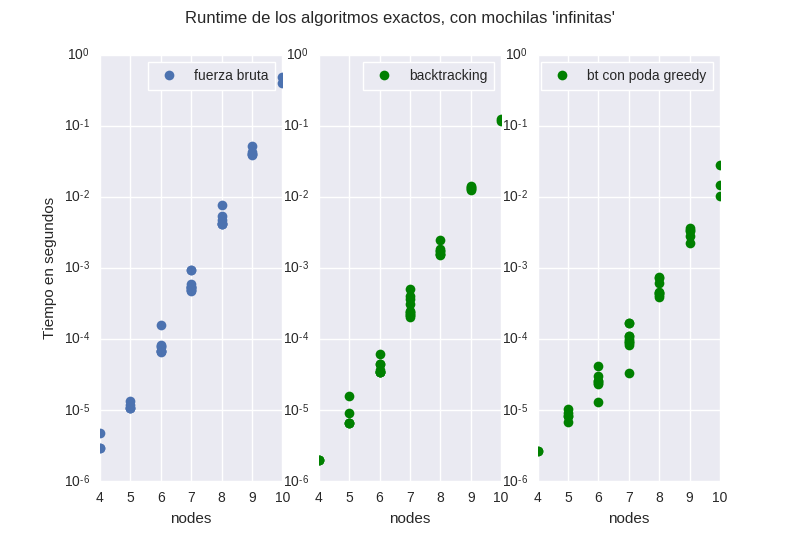
\includegraphics[width=14cm]{time-exacto}
    \caption{Tiempo de ejecución de los algoritmos exactos}
    \label{fig:time-exacto}
\end{figure}

\subsubsection{En función del tamaño de la mochila}

A continuación realizamos pruebas fijando la cantidad de gimnasios y paradas en 5 y variando el tamaño de la mochila.

Desafortunadamente vemos en la figura \ref{fig:time-exacto-moch} que dentro del intervalo de tamaños de mochila
interesantes, limitado por la cantidad de nodos que puede tener un problema a ser resuelto en un tiempo factible
(ya que si el tamaño es mayor a tres veces la cantidad de paradas, no influirá en el comportamiento del algoritmo),
no podemos determinar propiamente el comportamiento.

\begin{figure}[H]
    \centering
    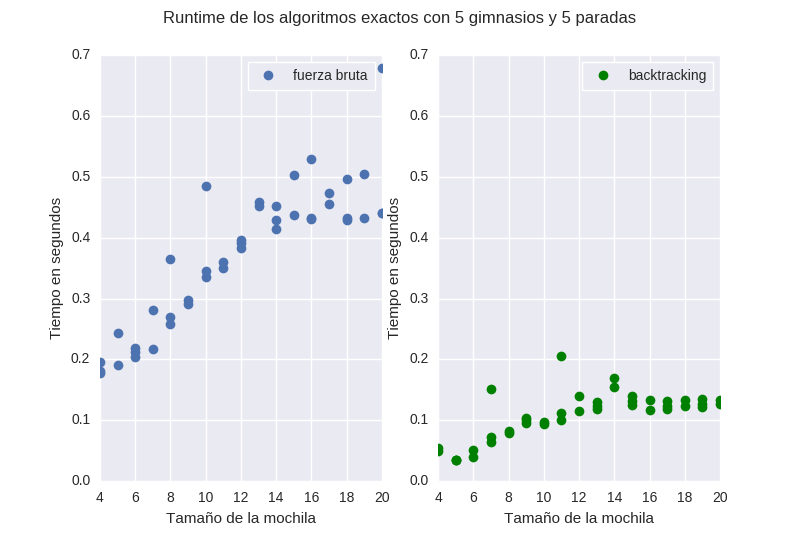
\includegraphics[width=13.5cm]{time-exacto-moch}
    \caption{Tiempo de ejecución de los algoritmos exactos al variar el tamaño de la mochila}
    \label{fig:time-exacto-moch}
\end{figure}

\subsection{Runtime de las heurísticas greedy}

\subsubsection{En función de la cantidad de nodos}

Medimos el tiempo en la figura \ref{fig:time-greedy} generando 5 casos para cada combinación de entre 1000 y 10000 gimnasios y paradas, avanzando de a 1000, y tamaño de mochila mayor a 30000.

Vemos en la figura \ref{fig:time-greedy-correlation} que estos tiempos tiempos se correlaciona fuertemente con un comportamiento cuadrático en función de la cantidad de nodos.

\begin{figure}[H]
    \centering
    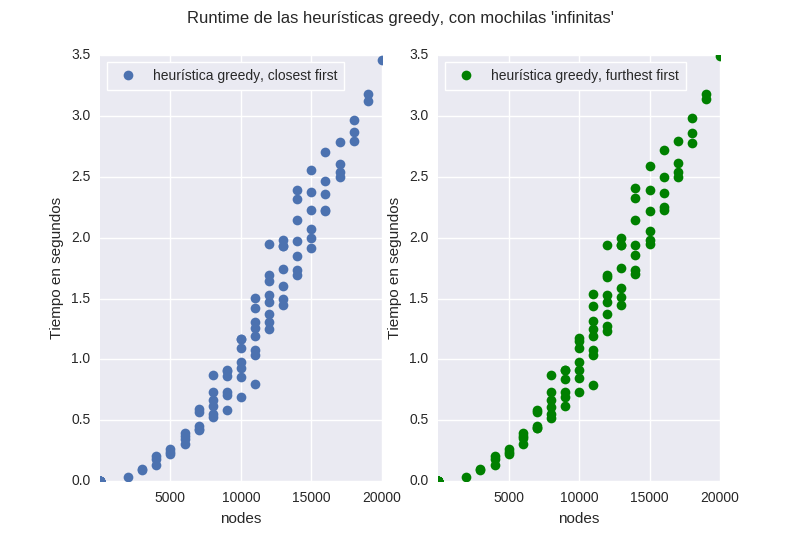
\includegraphics[width=13.5cm]{time-greedy}
    \caption{Tiempo de ejecución de las heurísticas greedy}
    \label{fig:time-greedy}
\end{figure}

\begin{figure}[H]
    \centering
    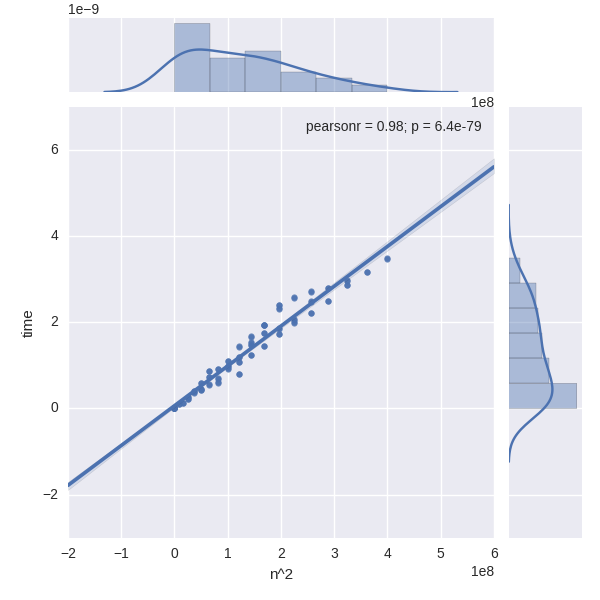
\includegraphics[width=10cm]{time-greedy-correlation}
    \caption{Correlación entre el tiempo de ejecución del greedy y una complejidad cuadrática}
    \label{fig:time-greedy-correlation}
\end{figure}

\subsubsection{En función del tamaño de la mochila}

Realizamos también pruebas fijando la cantidad de gimnasios y paradas en 2500 y variando el tamaño de la mochila entre 100 y 7500 en pasos de a 100, y nos encontramos con un comportamiento constante y con poco ruido para ambos tipos de greedy (con una correlación entre tiempo medido y tamaño de mochila de $0.170856$).

En el cuadro \ref{tab:time-greedy-moch} se encuentra una descripción de los datos medidos.

\begin{table}[H]
    \begin{center}
        \begin{tabular}{ l | r }
            count  & 76.000000 \\
            mean   &  0.215175 \\
            std    &  0.005658 \\
            min    &  0.209863 \\
            25\%   &  0.212328 \\
            50\%   &  0.213131 \\
            75\%   &  0.215283 \\
            max    &  0.239380 \\
        \end{tabular}
        \caption{Descripción de las mediciones en función del tamaño de mochila}\label{tab:time-greedy-moch}
    \end{center}
\end{table}

\subsection{Runtime de las heurísticas locales}

\subsubsection{En función de la cantidad de nodos}

Para las heurísticas locales medimos nuevamente los tiempos generando 5 casos para cada combinación de entre 10 y 100 gimnasios y paradas, avanzando de a 10, y tamaño de mochila mayor a 300. Los resultados se pueden apreciar en la figura \ref{fig:time-local}.

Podemos corroborar en la figura \ref{fig:time-local-correlation} que ambas variaciones se corresponden con un comportamiento de orden cuarto en función de la cantidad de nodos.

\begin{figure}[H]
    \centering
    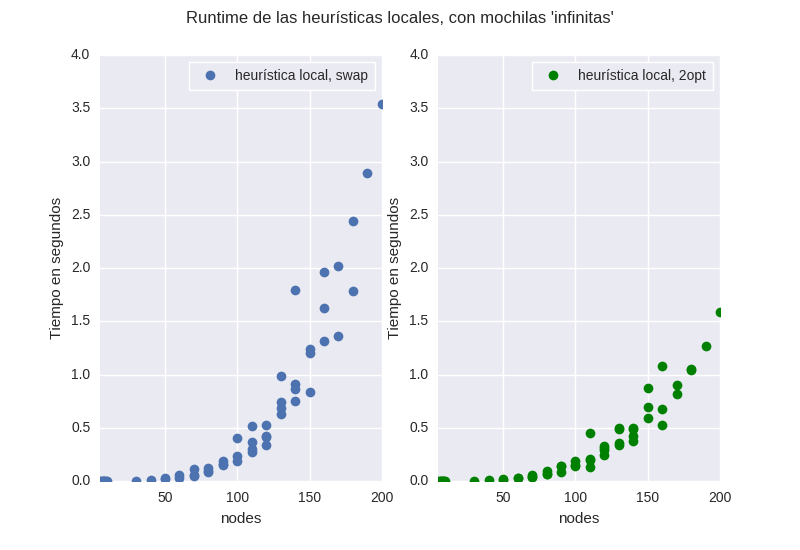
\includegraphics[width=13.5cm]{time-local}
    \caption{Tiempo de ejecución de las heurísticas locales}
    \label{fig:time-local}
\end{figure}

\begin{figure}[H]
    \centering
    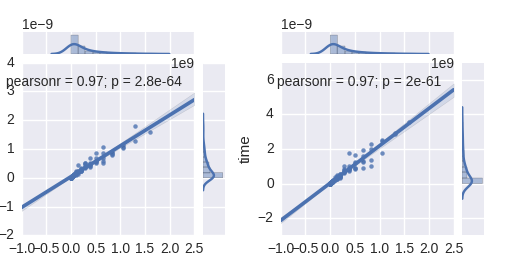
\includegraphics[width=13cm]{time-local-correlation}
    \caption{Correlación entre el tiempo de ejecución de las heurísticas locales 2opt (izquierda) y swap (derecha), con una complejidad $n^4$}
    \label{fig:time-local-correlation}
\end{figure}

\subsubsection{En función del tamaño de la mochila}

Nuevamente realizamos pruebas fijando la cantidad de gimnasios y paradas en 50 y variando el tamaño de la mochila entre 10 y 150, y nos encontramos, al igual que con el greedy, con un comportamiento constante en función de la mochila para ambas variaciones (con una correlación entre tiempo medido y tamaño de mochila de $0.259633$ para swap y de $0.265672$ para 2opt).

En el cuadro \ref{tab:time-local-moch} se encuentra una descripción de los datos medidos.

\begin{table}[H]
    \begin{center}
        \begin{tabular}{ l | r r }
            & Swap & 2opt \\
            \hline
            count  & 141.000000 & 141.000000 \\
            mean   &   0.263016 &   0.167931 \\
            std    &   0.080163 &   0.034468 \\
            min    &   0.124284 &   0.087849 \\
            25\%   &   0.214029 &   0.143264 \\
            50\%   &   0.253680 &   0.165566 \\
            75\%   &   0.297979 &   0.193758 \\
            max    &   0.566984 &   0.268200 \\
        \end{tabular}
        \caption{Descripción de las mediciones en función del tamaño de mochila}\label{tab:time-local-moch}
    \end{center}
\end{table}

\subsection{Runtime de la metaheurística GRASP}

\subsubsection{En función de la cantidad de nodos}

Para medir el comportamiento de GRASP generamos 4 instancias para cada combinación de gimnasios y mochilas entre 10 y 50, avanzando de a 5, con un tamaño de mochila superior a 150. En la figura \ref{fig:time-grasp} pueden apreciarse los resultados. Como se observa en la figura \ref{fig:time-grasp-correlation}, el comportamiento está fuertemente correlacionado a un orden 5 sobre la cantidad de nodos.

\begin{figure}[H]
    \centering
    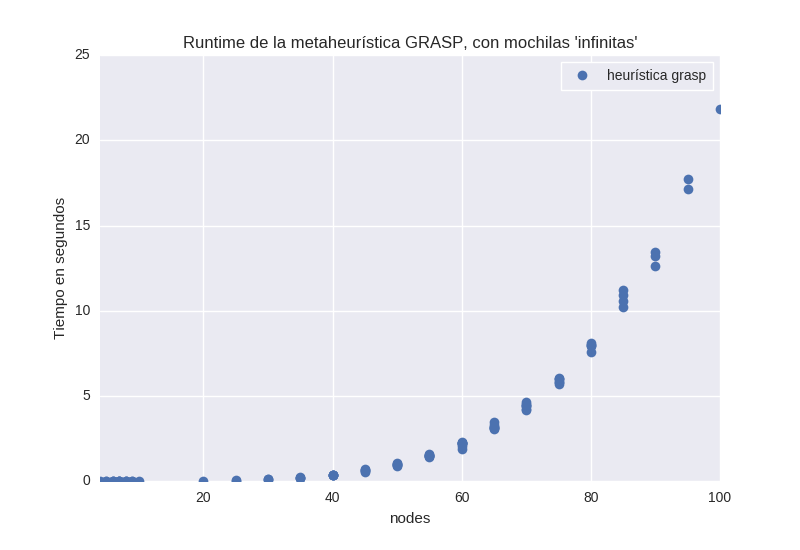
\includegraphics[width=13.5cm]{time-grasp}
    \caption{Tiempo de ejecución de la metaheurística grasp}
    \label{fig:time-grasp}
\end{figure}

\begin{figure}[H]
    \centering
    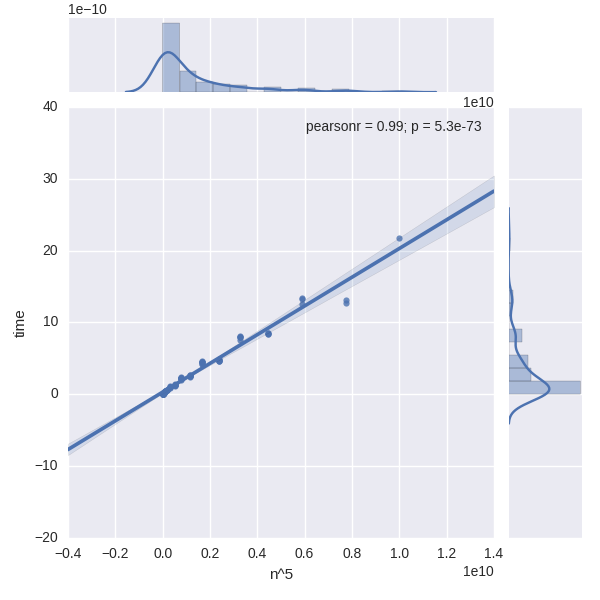
\includegraphics[width=10cm]{time-grasp-correlation}
    \caption{Correlación entre el tiempo de ejecución de grasp y una complejidad de orden 5 en función de la cantidad de nodos}
    \label{fig:time-grasp-correlation}
\end{figure}

\subsubsection{En función del tamaño de la mochila}

Para medir el tiempo de ejecución en función del tamaño de la mochila fijamos la cantidad de gimnasios y paradas en 20 y variamos la mochila entre 10 y 60. Como se aprecia en la figura \ref{fig:time-grasp-moch}, nos encontramos con que para tamaños pequeños se observa una correlación entre la mochila y el tiempo de ejecución, pero mas o menos a partir del tamaño 30 los tiempos se mantienen relativamente constantes.

Esto puede deberse a que cuando hay poco espacio el la mochila se limita la cantidad de opciones que puede tomar el algoritmo, lo que hace que termine mas temprano.

\begin{figure}[H]
    \centering
    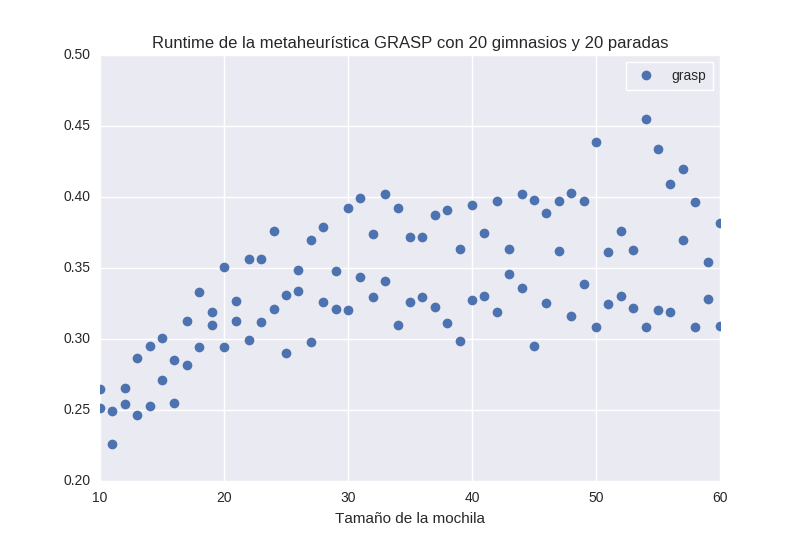
\includegraphics[width=11cm]{time-grasp-moch}
    \caption{Correlación entre el tiempo de ejecución de grasp y una complejidad de orden 5 en función de la cantidad de nodos}
    \label{fig:time-grasp-moch}
\end{figure}

\subsection{Precisión de las heurísticas}

Para medir que tan buenos son los resultados corrimos el mismo problema con cada heurística y comparamos con el resultado real,
obteniendo la proporción entre la solución encontrada y la buscada. Como el nuestro es un problema de minimización,
las proporciones siempre serán mayores o iguales a 1 (nuestras heurísticas siempre encuentran una solución posible).

Para testear problemas de mayor tamaño, tomamos como resultado de comparación el menor valor encontrado entre todas las heurísticas.

\subsubsection{Precisión en casos pequeños, comparando con el exacto}
\label{sec:precision-small}

Para cada combinación de gimnasios y paradas tal que su suma sea menor a 14 (y ambos $\geq 1$) generamos 4 casos usando el generador \texttt{random},
uno con mochila de tamaño 3, otro con tamaño igual a la cantidad de paradas, otro con el doble de las paradas
y uno con espacio igual a trues veces la cantidad de paradas.
Resolvimos estos casos con cada uno de nuestros algoritmos y comparamos las soluciones.

En la figura \ref{fig:precision-small-all} vemos las distribuciones de las precisiones para cada heurística.

Como era de esperar los algoritmos greedy suelen obtener resultados muy por encima del valor óptimo, aunque vemos que en el $75\%$
de los casos la variante closest first obtuvo un valor menor al doble del buscado.
Las heurísticas locales, especialmente la variante swap, mejoraron bastante la precision (a costa de un tiempo de ejecución bastante mas elevado).

Y por último, el GRASP obtuvo el óptimo en un $82.3\%$ de los casos.
En el cuadro \ref{tab:precision-small-grasp} se describe la distribución de su precisión.

\begin{figure}[H]
    \centering
    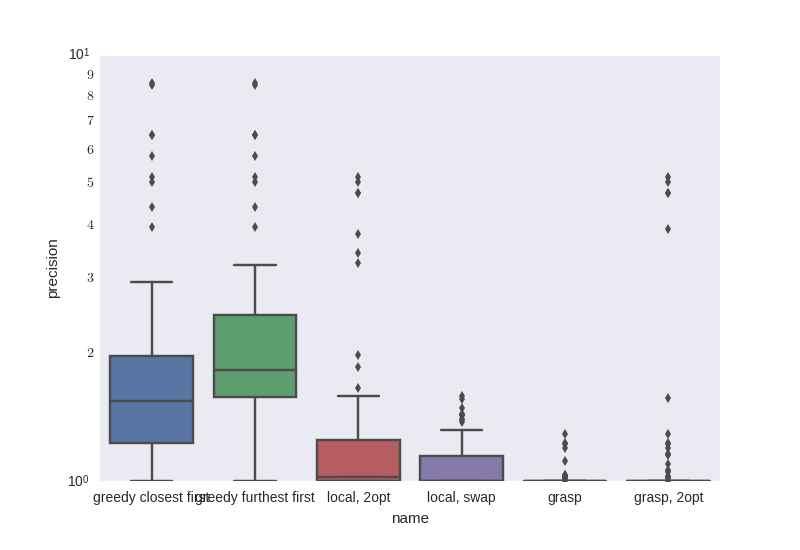
\includegraphics[width=12cm]{precision-small-all}
    \caption{Precisión comparando con el valor exacto}
    \label{fig:precision-small-all}
\end{figure}

\begin{table}[H]
    \begin{center}
        \begin{tabular}{ l | r }
            count  & 226.000000 \\
            mean   &   1.011650 \\
            std    &   0.039716 \\
            min    &   1.000000 \\
            25\%   &   1.000000 \\
            50\%   &   1.000000 \\
            75\%   &   1.000000 \\
            max    &   1.288691 \\
        \end{tabular}
        \caption{Descripción de la precisión de la metaheurística GRASP}\label{tab:precision-small-grasp}
    \end{center}
\end{table}

\subsubsection{Precisión en casos grandes, comparando con el mínimo}
\label{sec:precision-big}

A continuación generamos casos de prueba utilizando el generador \texttt{random} para todas las combinaciones de paradas y gimnasios tal que ambos
sean mayor o iguales a $10$ y su suma sea a lo sumo 40.
En cada caso variamos el tamaño de la mochila de igual forma que en la sección \ref{sec:precision-small}.

Nuevamente observamos como la variante closest first del greedy produce mejores resultados que la otra.

Además notamos que, si bien la heurística local swap no suele producir resultados muy malos,
su media es bastante peor que la variante 2opt, cuyos valores se describen en el cuadro \ref{tab:precision-big-local-2opt}.

Por último, la metaheurística grasp obtiene el mejor resultado en el $96.72\%$ de los casos.
Este número no es $100\%$ ya que existen casos donde los locales obtienen un buen resultado a partir del greedy closest first
pero el grasp, por la característica aleatoria de su ejecución, termina en una solución peor.

\begin{figure}[H]
    \centering
    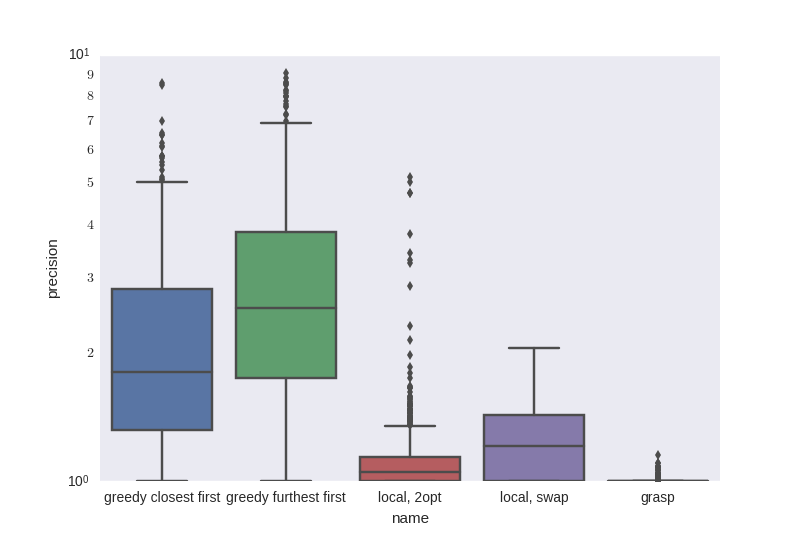
\includegraphics[width=12cm]{precision-big-all}
    \caption{Precisión comparando con el valor exacto}
    \label{fig:precision-big-all}
\end{figure}

\begin{table}[H]
    \begin{center}
        \begin{tabular}{ l | r }
            count  & 2008.000000 \\
            mean   &    1.111849 \\
            std    &    0.247017 \\
            min    &    1.000000 \\
            25\%   &    1.000000 \\
            50\%   &    1.049093 \\
            75\%   &    1.139941 \\
            max    &    5.181492 \\
        \end{tabular}
        \caption{Descripción de la precisión de la heurística local 2opt}\label{tab:precision-big-local-2opt}
    \end{center}
\end{table}

\subsubsection{Precisión en función del generador}

Utilizando las mismas variables descriptas en la sección \ref{sec:precision-big} generamos instancias con cada uno de los generadores
disponibles, para ver si la precisión variaba con los tipos de problema.

El resultado puede verse en la figura \ref{fig:precision-big-all-bygen}.
Para las instancias de \ref{zigzag} se suele conseguir buenos resultados en comparación con las \texttt{random}.
Ademas es notable que las instancias de \texttt{separated} se suelen resolver relativamente bien con las heurísticas locales y GRASP,
no así con los greedy.

\begin{figure}[H]
    \centering
    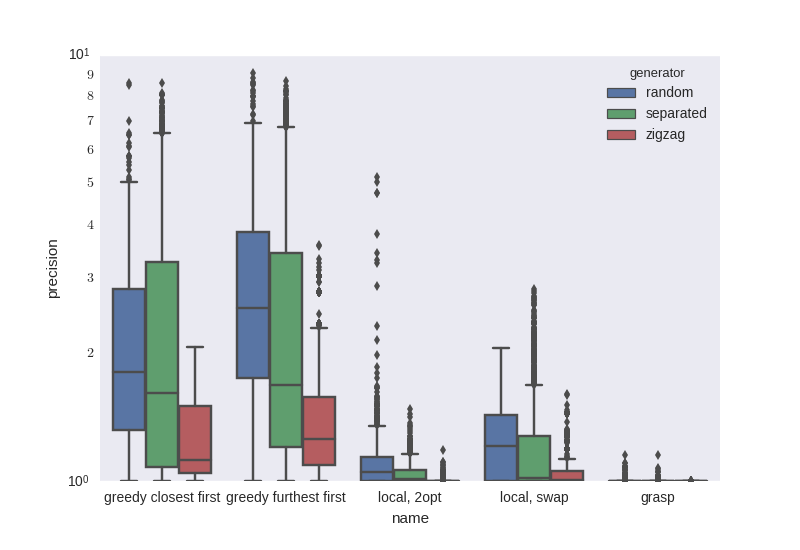
\includegraphics[width=12cm]{precision-big-all-bygen}
    \caption{Precisión comparando con el mínimo, según el generador utilizado}
    \label{fig:precision-big-all-bygen}
\end{figure}

\subsubsection{Precisión en función del tamaño de la mochila}

Quisimos también probar si el tamaño de las mochilas influía en la precisión de cada método.
Para ello tomamos los resultados obtenidos en la sección \ref{sec:precision-big} y los separamos
por el tamaño de la mochila relativo a la cantidad de paradas.

El resultado, que puede observarse en la figura \ref{fig:precision-big-all-bysize},
muestra una leve correlación para las heurísticas greedy. Las heurísticas locales y GRASP, en cambio, no parecen verse afectadas.

\begin{figure}[H]
    \centering
    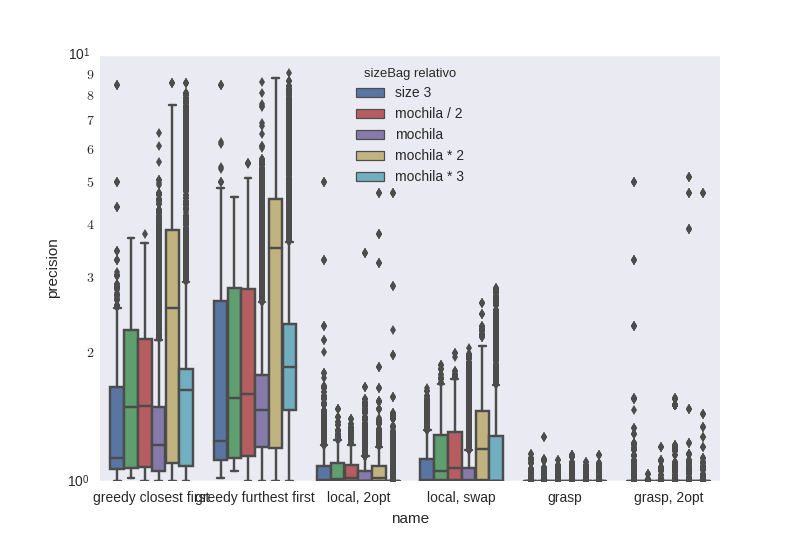
\includegraphics[width=12cm]{precision-big-all-bysize}
    \caption{Precisión comparando con el mínimo, según el tamaño relativo de la mochila}
    \label{fig:precision-big-all-bysize}
\end{figure}


%\newpage
%\section{Códigos Fuente}
\subsection{Ejercicio 1}

\lstset{language=C++,
                basicstyle=\ttfamily,
                keywordstyle=\color{blue}\ttfamily,
                stringstyle=\color{red}\ttfamily,
                commentstyle=\color{green}\ttfamily,
                morecomment=[l][\color{magenta}]{\#}
}

\begin{lstlisting}[ basicstyle=\small]
    #include <math.h>
    #include <stdint.h>
    #include <algorithm>
    #include <cassert>
    #include <iostream>
    #include <map>
    #include <queue>
    #include <set>
    #include <tuple>
    #include <vector>

    using namespace std;

    // Hay 2^(N+M) estados posibles
    typedef struct estado_t {
        // Para todo, true = del lado derecho
        vector<bool> arq;
        vector<bool> can;
        bool linterna = false;

        estado_t(){};
        estado_t(uint32_t n, uint32_t m) : arq(n), can(m) {}

        // La priority_queue requiere <
        bool operator<(const struct estado_t &o) const {
            return tie(linterna, arq, can) < tie(o.linterna, o.arq, o.can);
        }
        bool operator==(const struct estado_t &o) const {
            return tie(linterna, arq, can) == tie(o.linterna, o.arq, o.can);
        }
    } estado;

    vector<uint32_t> arq;
    vector<uint32_t> can;

    bool agregarCandidato(map<estado, uint32_t> &dist,
                          set<pair<uint32_t, estado>> &candidatos, estado &hijo,
                          uint32_t peso);

    int64_t tiempoMinimo(const vector<uint32_t> &arq, const vector<uint32_t> &can) {
        // Empiezan todos del lado izquierdo
        estado inicial(arq.size(), can.size());
        estado objetivo;
        objetivo.arq = vector<bool>(arq.size(), true);
        objetivo.can = vector<bool>(can.size(), true);
        objetivo.linterna = true;

        // Distancia minima hasta el estado
        map<estado, uint32_t> dist;
        dist.insert({inicial, 0});

        // Mantenemos la lista de candidatos a explorar,
        // y vemos siempre el mas cercano primero
        set<pair<uint32_t, estado>> candidatos;
        candidatos.insert(make_pair(0, inicial));

        int64_t res = -1;
        while (!candidatos.empty()) {
            auto p = candidatos.begin();
            uint32_t costo = p->first;
            estado nodo = p->second;
            candidatos.erase(p);

            // Llegamos a la solucion
            if (nodo == objetivo) {
                res = costo;
                break;
            }

            // Hacemos un population count
            uint32_t arqIzq = 0;
            uint32_t canIzq = 0;

            for (uint32_t i = 0; i < arq.size(); i++)
                if (nodo.arq[i])
                    arqIzq++;
            for (uint32_t i = 0; i < can.size(); i++)
                if (nodo.can[i])
                    canIzq++;

            // Checkeamos que no sea un caso invalido
            if ((arq.size() - arqIzq > 0) &&
                (arq.size() - arqIzq) < (can.size() - canIzq)) {
                continue;
            }
            if (arqIzq > 0 && arqIzq < canIzq) {
                continue;
            }

            // Generamos los pasos posibles a partir de donde estamos
            estado hijo = nodo;
            hijo.linterna = !hijo.linterna;

            for (uint32_t i = 0; i < arq.size(); i++) {
                // Checkear si esta de este lado
                if (nodo.arq[i] != nodo.linterna)
                    continue;

                hijo.arq[i] = !nodo.linterna;
                for (uint32_t j = i; j < arq.size(); j++) {
                    if (nodo.arq[j] != nodo.linterna)
                        continue;
                    hijo.arq[j] = !nodo.linterna;

                    // El movimiento siempre cuesta la menor de las velocidades
                    uint32_t costoExtra = max(arq[i], arq[j]);
                    uint32_t distancia = costo + costoExtra;

                    // Agregamos este hijo a la lista
                    agregarCandidato(dist, candidatos, hijo, distancia);

                    if (i != j)
                        hijo.arq[j] = nodo.linterna;
                }
                // Lo volvemos a como estaba
                hijo.arq[i] = nodo.linterna;
            }

            for (uint32_t i = 0; i < can.size(); i++) {
                // Checkear si esta de este lado
                if (nodo.can[i] != nodo.linterna)
                    continue;

                hijo.can[i] = !nodo.linterna;
                for (uint32_t j = i; j < can.size(); j++) {
                    if (nodo.can[j] != nodo.linterna)
                        continue;
                    hijo.can[j] = !nodo.linterna;

                    // El movimiento siempre cuesta la menor de las velocidades
                    uint32_t costoExtra = max(can[i], can[j]);
                    uint32_t distancia = costo + costoExtra;

                    // Agregamos este hijo a la lista
                    agregarCandidato(dist, candidatos, hijo, distancia);

                    if (i != j)
                        hijo.can[j] = nodo.linterna;
                }
                // Lo volvemos a como estaba
                hijo.can[i] = nodo.linterna;
            }

            for (uint32_t i = 0; i < arq.size(); i++) {
                // Checkear si esta de este lado
                if (nodo.arq[i] != nodo.linterna)
                    continue;

                hijo.arq[i] = !nodo.linterna;
                for (uint32_t j = 0; j < can.size(); j++) {
                    if (nodo.can[j] != nodo.linterna)
                        continue;
                    hijo.can[j] = !nodo.linterna;

                    // El movimiento siempre cuesta la menor de las velocidades
                    uint32_t costoExtra = max(arq[i], can[j]);
                    uint32_t distancia = costo + costoExtra;

                    // Agregamos este hijo a la lista
                    agregarCandidato(dist, candidatos, hijo, distancia);

                    hijo.can[j] = nodo.linterna;
                }
                // Lo volvemos a como estaba
                hijo.arq[i] = nodo.linterna;
            }
        }

        return res;
    }
\end{lstlisting}
\begin{lstlisting}[ basicstyle=\small]
    bool agregarCandidato(map<estado, uint32_t> &dist,
                          set<pair<uint32_t, estado>> &candidatos, estado &hijo,
                          uint32_t distancia) {
        auto s = dist.find(hijo);
        if (s != dist.end()) {
            // El hijo ya tiene una distancia
            // lo agregamos solo si la distancia resultante es menor
            uint32_t distVieja = s->second;

            if (distancia < distVieja) {
                // Hay que borrar la posicion en la cola de candidatos
                // para insertarlo de nuevo
                auto p = candidatos.find({distVieja, hijo});
                candidatos.erase(p);
                dist.erase(dist.find(hijo));
            } else {
                // La distancia anterior ya era mejor que venir por este camino
                return false;
            }
        }

        dist.insert({hijo, distancia});
        candidatos.insert({distancia, hijo});

        return true;
    }
\end{lstlisting}

\newpage
%-------------------------------------------------------------------
%-------------------------------------------------------------------
%-------------------------------------------------------------------
\subsection{Ejercicio 2}

\begin{lstlisting}[ basicstyle=\small]
      #include <math.h>
      #include <stdint.h>
      #include <iostream>
      #include <set>
      #include <vector>

      using namespace std;

      uint64_t peso;

      void balancear(uint64_t peso, vector<uint8_t> &izq, vector<uint8_t> &der) {
          // peso = sum(3^izq) - sum(3^der)

          bool carry = false;
          uint8_t exponente = 0;

          // Recorremos los dígitos en base 3, empezando por el menos significativo
          while (peso > 0) {
              uint8_t digito = peso % 3;
              peso /= 3;

              // Le sumamos una pesa al dígito anterior, y quedo un carry
              if (carry) {
                  digito += 1;
                  digito %= 3;

                  // Checkear si se genero otro carry mas
                  carry = digito == 0;
              }

              if (digito == 2) {
                  // A cada dígito '2' del peso hay que sumarle 1

                  // Agregamos una pesa con este exponente
                  der.push_back(exponente);

                  // Actualizamos el peso
                  digito = 0;
                  carry = true;

              } else if (digito == 1) {
                  // Si quedo un 1 agregamos una pesa del otro lado, para
                  // contrarestarlo
                  izq.push_back(exponente);
              }

              exponente++;
          }

          if (carry)
              izq.push_back(exponente);
      }
\end{lstlisting}

\newpage
%-------------------------------------------------------------------
%-------------------------------------------------------------------
%-------------------------------------------------------------------
\subsection{Ejercicio 3}

\begin{lstlisting}[ basicstyle=\small]
#include <stdint.h>
#include <algorithm>
#include <iostream>
#include <map>
#include <set>
#include <vector>
#include <math.h>

using namespace std;

typedef struct mkp_object_t {
    uint64_t id;
    uint64_t weight;
    int64_t value;
} mkp_object;

vector<uint64_t> bins(3,0);
vector<mkp_object> objects;

uint64_t mkp(vector<uint64_t> bins, vector<mkp_object> const &objetos,
             vector<vector<uint64_t>> &resultIds) {
    // O(pi(bins) * count(objects) )

    // Si hay menos de 3 mochilas, consideramos las siguientes como
    // de tamano 0

    // Para cada combinacion de k_i pesos de las mochilas, con 0 <= k_i <=
    // capacidad(i)
    // calculamos el mayor valor conseguible ocupando exactamente ese espacio
    //
    // En cada combinacion, para cada 0 <= j <= cantidad de objetos,
    // calculamos el optimo usando los primeros j objetos.

    vector<vector<vector<vector<int64_t>>>> mejorValor(
        bins[0] + 1,
        vector<vector<vector<int64_t>>>(
            bins[1] + 1,
            vector<vector<int64_t>>(bins[2] + 1,
                                    vector<int64_t>(objetos.size() + 1, -1))));

    vector<vector<vector<vector<int64_t>>>> binObjeto(
        bins[0] + 1,
        vector<vector<vector<int64_t>>>(
            bins[1] + 1,
            vector<vector<int64_t>>(bins[2] + 1,
                                    vector<int64_t>(objetos.size() + 1, -1))));

    // 0 objetos en mochilas de tamano 0 tienen valor 0
    mejorValor[0][0][0][0] = 0;

    int64_t valorMax = 0;
    vector<uint64_t> sizesMax(3, 0);

    for (uint64_t w0 = 0; w0 <= bins[0]; w0++) {
        for (uint64_t w1 = 0; w1 <= bins[1]; w1++) {
            for (uint64_t w2 = 0; w2 <= bins[2]; w2++) {
                // Para cada primeros j objetos buscamos el máximo
                for (uint64_t j = 1; j <= objetos.size(); j++) {
                    const mkp_object &obj = objetos[j - 1];

                    // Decidimos si conviene poner el objeto en una mochila o no
                    // usarlo
                    int64_t valCandidato, valor = mejorValor[w0][w1][w2][j - 1];

                    valCandidato = obj.weight > w0 ? -1 :
                        mejorValor[w0 - obj.weight][w1][w2][j - 1] + obj.value;
                    if (valor < valCandidato) {
                        binObjeto[w0][w1][w2][j] = 0;
                        valor = valCandidato;
                    }

                    valCandidato = obj.weight > w1 ? -1 :
                        mejorValor[w0][w1 - obj.weight][w2][j - 1] + obj.value;
                    if (valor < valCandidato) {
                        binObjeto[w0][w1][w2][j] = 1;
                        valor = valCandidato;
                    }

                    valCandidato = obj.weight > w2 ? -1 :
                        mejorValor[w0][w1][w2 - obj.weight][j - 1] + obj.value;
                    if (valor < valCandidato) {
                        binObjeto[w0][w1][w2][j] = 2;
                        valor = valCandidato;
                    }

                    mejorValor[w0][w1][w2][j] = valor;
                }

                // Mantenemos el máximo valor visto
                if (valorMax < mejorValor[w0][w1][w2][objetos.size()]) {
                    valorMax = mejorValor[w0][w1][w2][objetos.size()];
                    sizesMax = {w0, w1, w2};
                }
            }
        }
    }

    // Escribimos los ids del resultado
    resultIds.resize(bins.size());

    for(uint64_t j=objetos.size(); j > 0; j--) {
        int64_t bin = binObjeto[sizesMax[0]][sizesMax[1]][sizesMax[2]][j];
        if (bin != -1) {
            resultIds[bin].push_back(objetos[j-1].id);
            sizesMax[bin] -= objetos[j-1].weight;
        }
    }

    // Como recorrimos los objetos desde el ultimo hay que invertir el array
    // (se pide ordenado)
    for (auto &v : resultIds) {
        reverse(v.begin(), v.end());
    }
    return valorMax;
}
\end{lstlisting}


\appendix

%\newpage
%\bibliography{bibliography}{}
%\bibliographystyle{plain}

\end{document}
